\documentclass{book}
\usepackage[a4paper,top=2.5cm,bottom=2.5cm,left=2.5cm,right=2.5cm]{geometry}
\usepackage{makeidx}
\usepackage{natbib}
\usepackage{graphicx}
\usepackage{multicol}
\usepackage{float}
\usepackage{listings}
\usepackage{color}
\usepackage{ifthen}
\usepackage[table]{xcolor}
\usepackage{textcomp}
\usepackage{alltt}
\usepackage{ifpdf}
\ifpdf
\usepackage[pdftex,
            pagebackref=true,
            colorlinks=true,
            linkcolor=blue,
            unicode
           ]{hyperref}
\else
\usepackage[ps2pdf,
            pagebackref=true,
            colorlinks=true,
            linkcolor=blue,
            unicode
           ]{hyperref}
\usepackage{pspicture}
\fi
\usepackage[utf8]{inputenc}
\usepackage{mathptmx}
\usepackage[scaled=.90]{helvet}
\usepackage{courier}
\usepackage{sectsty}
\usepackage{amssymb}
\usepackage[titles]{tocloft}
\usepackage{doxygen}
\lstset{language=C++,inputencoding=utf8,basicstyle=\footnotesize,breaklines=true,breakatwhitespace=true,tabsize=4,numbers=left }
\makeindex
\setcounter{tocdepth}{3}
\renewcommand{\footrulewidth}{0.4pt}
\renewcommand{\familydefault}{\sfdefault}
\hfuzz=15pt
\setlength{\emergencystretch}{15pt}
\hbadness=750
\tolerance=750
\begin{document}
\hypersetup{pageanchor=false,citecolor=blue}
\begin{titlepage}
\vspace*{7cm}
\begin{center}
{\Large Assignment 3 -\/ Breakout \\[1ex]\large 1 }\\
\vspace*{1cm}
{\large Generated by Doxygen 1.8.3.1}\\
\vspace*{0.5cm}
{\small Thu May 29 2014 14:46:31}\\
\end{center}
\end{titlepage}
\clearemptydoublepage
\pagenumbering{roman}
\tableofcontents
\clearemptydoublepage
\pagenumbering{arabic}
\hypersetup{pageanchor=true,citecolor=blue}
\chapter{I\-N\-F\-O3220 -\/ Assignment Stage 2}
\label{md_README}
\hypertarget{md_README}{}
\subsection*{A\-S\-S\-U\-M\-P\-T\-I\-O\-N\-S}


\begin{DoxyItemize}
\item Default values such as the location of the config file are stored in the \hyperlink{defaults_8h_source}{defaults.\-h}. This may need to be modified to execute.
\end{DoxyItemize}

\subsection*{D\-E\-S\-I\-G\-N P\-A\-T\-T\-E\-R\-N}

The {\itshape structural} design pattern used in this program is {\bfseries Apdater} pattern. It was used on the config class, as an adapter to a vector container. The config class contains many different config items and can be extentend to include others.

\subsection*{E\-X\-T\-E\-N\-S\-I\-O\-N}


\begin{DoxyItemize}
\item You can add extra blocks by left-\/clicking in the box.
\item You can add extra balls by right-\/clicking in the box.
\item Any new items are given the default values found in \hyperlink{defaults_8h_source}{defaults.\-h}.
\item Balls have correct elastic collisions.
\item The bricks change colour as their lives diminish.
\item You can specify the hue of each item, block or ball using the color\-Hue 
\end{DoxyItemize}
\chapter{Hierarchical Index}
\section{Class Hierarchy}
This inheritance list is sorted roughly, but not completely, alphabetically\-:\begin{DoxyCompactList}
\item \contentsline{section}{Abstract\-Responsibility}{\pageref{classAbstractResponsibility}}{}
\begin{DoxyCompactList}
\item \contentsline{section}{Dialog}{\pageref{classDialog}}{}
\item \contentsline{section}{Help\-Dialog\-Manager}{\pageref{classHelpDialogManager}}{}
\item \contentsline{section}{Level}{\pageref{classLevel}}{}
\item \contentsline{section}{Paddle}{\pageref{classPaddle}}{}
\item \contentsline{section}{Score\-Board\-Manager}{\pageref{classScoreBoardManager}}{}
\end{DoxyCompactList}
\item \contentsline{section}{Chain\-Of\-Responsibility}{\pageref{classChainOfResponsibility}}{}
\item \contentsline{section}{Config}{\pageref{classConfig}}{}
\item \contentsline{section}{Config\-Item}{\pageref{classConfigItem}}{}
\begin{DoxyCompactList}
\item \contentsline{section}{Ball\-Config\-Item}{\pageref{classBallConfigItem}}{}
\item \contentsline{section}{Block\-Config\-Item}{\pageref{classBlockConfigItem}}{}
\item \contentsline{section}{Level\-Config\-Item}{\pageref{classLevelConfigItem}}{}
\item \contentsline{section}{Paddle\-Config\-Item}{\pageref{classPaddleConfigItem}}{}
\end{DoxyCompactList}
\item \contentsline{section}{Event}{\pageref{classEvent}}{}
\begin{DoxyCompactList}
\item \contentsline{section}{Ball\-Lost\-Event}{\pageref{classBallLostEvent}}{}
\item \contentsline{section}{Block\-Deleted\-Event}{\pageref{classBlockDeletedEvent}}{}
\item \contentsline{section}{Key\-Event}{\pageref{classKeyEvent}}{}
\item \contentsline{section}{Level\-Cleared\-Event}{\pageref{classLevelClearedEvent}}{}
\item \contentsline{section}{Out\-Of\-Lives\-Event}{\pageref{classOutOfLivesEvent}}{}
\end{DoxyCompactList}
\item \contentsline{section}{Item\-Factory}{\pageref{classItemFactory}}{}
\item Q\-Dialog\begin{DoxyCompactList}
\item \contentsline{section}{Dialog}{\pageref{classDialog}}{}
\end{DoxyCompactList}
\item Q\-Graphics\-Ellipse\-Item\begin{DoxyCompactList}
\item \contentsline{section}{Ball}{\pageref{classBall}}{}
\end{DoxyCompactList}
\item Q\-Graphics\-Rect\-Item\begin{DoxyCompactList}
\item \contentsline{section}{Block}{\pageref{classBlock}}{}
\item \contentsline{section}{Paddle}{\pageref{classPaddle}}{}
\end{DoxyCompactList}
\item Q\-Graphics\-Simple\-Text\-Item\begin{DoxyCompactList}
\item \contentsline{section}{Score}{\pageref{classScore}}{}
\end{DoxyCompactList}
\item \contentsline{section}{qt\-\_\-meta\-\_\-stringdata\-\_\-\-Dialog\-\_\-t}{\pageref{structqt__meta__stringdata__Dialog__t}}{}
\item \contentsline{section}{Ui\-\_\-\-Dialog}{\pageref{classUi__Dialog}}{}
\begin{DoxyCompactList}
\item \contentsline{section}{Ui\-:\-:Dialog}{\pageref{classUi_1_1Dialog}}{}
\end{DoxyCompactList}
\item \contentsline{section}{Ui\-\_\-help\-Dialog}{\pageref{classUi__helpDialog}}{}
\begin{DoxyCompactList}
\item \contentsline{section}{Ui\-:\-:help\-Dialog}{\pageref{classUi_1_1helpDialog}}{}
\end{DoxyCompactList}
\item \contentsline{section}{Ui\-\_\-high\-Scores}{\pageref{classUi__highScores}}{}
\begin{DoxyCompactList}
\item \contentsline{section}{Ui\-:\-:high\-Scores}{\pageref{classUi_1_1highScores}}{}
\end{DoxyCompactList}
\end{DoxyCompactList}

\chapter{Class Index}
\section{Class List}
Here are the classes, structs, unions and interfaces with brief descriptions\-:\begin{DoxyCompactList}
\item\contentsline{section}{\hyperlink{classAbstractResponsibility}{Abstract\-Responsibility} \\*Chain of responsibility participants base class }{\pageref{classAbstractResponsibility}}{}
\item\contentsline{section}{\hyperlink{classBall}{Ball} \\*The \hyperlink{classBall}{Ball} class }{\pageref{classBall}}{}
\item\contentsline{section}{\hyperlink{classBallConfigItem}{Ball\-Config\-Item} }{\pageref{classBallConfigItem}}{}
\item\contentsline{section}{\hyperlink{classBallLostEvent}{Ball\-Lost\-Event} \\*The ball was lost at the bottom }{\pageref{classBallLostEvent}}{}
\item\contentsline{section}{\hyperlink{classBlock}{Block} \\*The \hyperlink{classBlock}{Block} class }{\pageref{classBlock}}{}
\item\contentsline{section}{\hyperlink{classBlockConfigItem}{Block\-Config\-Item} }{\pageref{classBlockConfigItem}}{}
\item\contentsline{section}{\hyperlink{classBlockDeletedEvent}{Block\-Deleted\-Event} \\*Triggered when a block is removed from the scene }{\pageref{classBlockDeletedEvent}}{}
\item\contentsline{section}{\hyperlink{classChainOfResponsibility}{Chain\-Of\-Responsibility} \\*Traverse chain of responsibility and manage it }{\pageref{classChainOfResponsibility}}{}
\item\contentsline{section}{\hyperlink{classConfig}{Config} }{\pageref{classConfig}}{}
\item\contentsline{section}{\hyperlink{classConfigItem}{Config\-Item} }{\pageref{classConfigItem}}{}
\item\contentsline{section}{\hyperlink{classDialog}{Dialog} }{\pageref{classDialog}}{}
\item\contentsline{section}{\hyperlink{classUi_1_1Dialog}{Ui\-::\-Dialog} }{\pageref{classUi_1_1Dialog}}{}
\item\contentsline{section}{\hyperlink{classEvent}{Event} \\*The base structure for all events }{\pageref{classEvent}}{}
\item\contentsline{section}{\hyperlink{classUi_1_1helpDialog}{Ui\-::help\-Dialog} }{\pageref{classUi_1_1helpDialog}}{}
\item\contentsline{section}{\hyperlink{classHelpDialogManager}{Help\-Dialog\-Manager} \\*Display a window with a help text }{\pageref{classHelpDialogManager}}{}
\item\contentsline{section}{\hyperlink{classUi_1_1highScores}{Ui\-::high\-Scores} }{\pageref{classUi_1_1highScores}}{}
\item\contentsline{section}{\hyperlink{classItemFactory}{Item\-Factory} }{\pageref{classItemFactory}}{}
\item\contentsline{section}{\hyperlink{classKeyEvent}{Key\-Event} \\*Transport key stroke events }{\pageref{classKeyEvent}}{}
\item\contentsline{section}{\hyperlink{classLevel}{Level} \\*Implement levels and switching to next one }{\pageref{classLevel}}{}
\item\contentsline{section}{\hyperlink{classLevelClearedEvent}{Level\-Cleared\-Event} \\*Triggered when all blocks are removed from a scene }{\pageref{classLevelClearedEvent}}{}
\item\contentsline{section}{\hyperlink{classLevelConfigItem}{Level\-Config\-Item} \\*Store config-\/file data of a level }{\pageref{classLevelConfigItem}}{}
\item\contentsline{section}{\hyperlink{classOutOfLivesEvent}{Out\-Of\-Lives\-Event} \\*Triggered when the lives reaches zero }{\pageref{classOutOfLivesEvent}}{}
\item\contentsline{section}{\hyperlink{classPaddle}{Paddle} \\*Implement the paddle a the bottom of the screen }{\pageref{classPaddle}}{}
\item\contentsline{section}{\hyperlink{classPaddleConfigItem}{Paddle\-Config\-Item} \\*Store and propagate the paddle's configuration }{\pageref{classPaddleConfigItem}}{}
\item\contentsline{section}{\hyperlink{structqt__meta__stringdata__Dialog__t}{qt\-\_\-meta\-\_\-stringdata\-\_\-\-Dialog\-\_\-t} }{\pageref{structqt__meta__stringdata__Dialog__t}}{}
\item\contentsline{section}{\hyperlink{classScore}{Score} \\*Store the score in a game }{\pageref{classScore}}{}
\item\contentsline{section}{\hyperlink{classScoreBoardManager}{Score\-Board\-Manager} \\*Manage displaying the score board and name entry }{\pageref{classScoreBoardManager}}{}
\item\contentsline{section}{\hyperlink{classUi__Dialog}{Ui\-\_\-\-Dialog} }{\pageref{classUi__Dialog}}{}
\item\contentsline{section}{\hyperlink{classUi__helpDialog}{Ui\-\_\-help\-Dialog} }{\pageref{classUi__helpDialog}}{}
\item\contentsline{section}{\hyperlink{classUi__highScores}{Ui\-\_\-high\-Scores} }{\pageref{classUi__highScores}}{}
\end{DoxyCompactList}

\chapter{Class Documentation}
\hypertarget{classAbstractResponsibility}{\section{Abstract\-Responsibility Class Reference}
\label{classAbstractResponsibility}\index{Abstract\-Responsibility@{Abstract\-Responsibility}}
}


Chain of responsibility participants base class.  




{\ttfamily \#include $<$Abstract\-Responsibility.\-h$>$}

Inheritance diagram for Abstract\-Responsibility\-:\begin{figure}[H]
\begin{center}
\leavevmode
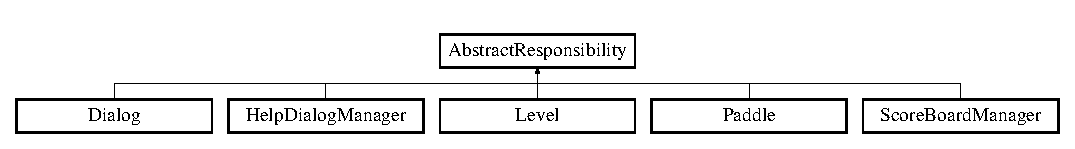
\includegraphics[height=1.555556cm]{classAbstractResponsibility}
\end{center}
\end{figure}
\subsection*{Public Member Functions}
\begin{DoxyCompactItemize}
\item 
\hyperlink{classAbstractResponsibility_ab11b9ec178012c0ab361ef4abe8be9e9}{Abstract\-Responsibility} ()
\item 
virtual \hyperlink{classAbstractResponsibility_af7ae360c861e5ba2e9024c830a3526c5}{$\sim$\-Abstract\-Responsibility} ()
\item 
void \hyperlink{classAbstractResponsibility_a9108e8a0a63112ef3077da388ed19eba}{add2\-Chain} (\hyperlink{classAbstractResponsibility}{Abstract\-Responsibility} $\ast$n)
\item 
virtual void \hyperlink{classAbstractResponsibility_a14d885884ae4841dbe7c5824b986f2c9}{handle\-Event} (\hyperlink{classEvent}{Event} $\ast$)
\end{DoxyCompactItemize}
\subsection*{Protected Attributes}
\begin{DoxyCompactItemize}
\item 
\hyperlink{classAbstractResponsibility}{Abstract\-Responsibility} $\ast$ \hyperlink{classAbstractResponsibility_a2af04f271483fd99267d5f6205ec257f}{next}
\end{DoxyCompactItemize}
\subsection*{Friends}
\begin{DoxyCompactItemize}
\item 
class \hyperlink{classAbstractResponsibility_a481df313240bacf48790db6d338f51d0}{Chain\-Of\-Responsibility}
\end{DoxyCompactItemize}


\subsection{Detailed Description}
Chain of responsibility participants base class. 

All objects that want to participate in the chain of responsibilities have to be derived from these class and implement the \hyperlink{classAbstractResponsibility_a14d885884ae4841dbe7c5824b986f2c9}{handle\-Event()} method. \hyperlink{classAbstractResponsibility_a14d885884ae4841dbe7c5824b986f2c9}{handle\-Event()} gets the event to handle and when the object decides to consume the event it just has to quit \hyperlink{classAbstractResponsibility_a14d885884ae4841dbe7c5824b986f2c9}{handle\-Event()}, if it does no consume event, then the base class' \hyperlink{classAbstractResponsibility_a14d885884ae4841dbe7c5824b986f2c9}{handle\-Event()} has to be called to enable propagation along the chain. This class in combination with \hyperlink{classChainOfResponsibility}{Chain\-Of\-Responsibility} implements the behavioural design pattern Chain Of Responsibility (p. 223 in Go\-F-\/book). 

\subsection{Constructor \& Destructor Documentation}
\hypertarget{classAbstractResponsibility_ab11b9ec178012c0ab361ef4abe8be9e9}{\index{Abstract\-Responsibility@{Abstract\-Responsibility}!Abstract\-Responsibility@{Abstract\-Responsibility}}
\index{Abstract\-Responsibility@{Abstract\-Responsibility}!AbstractResponsibility@{Abstract\-Responsibility}}
\subsubsection[{Abstract\-Responsibility}]{\setlength{\rightskip}{0pt plus 5cm}Abstract\-Responsibility\-::\-Abstract\-Responsibility (
\begin{DoxyParamCaption}
{}
\end{DoxyParamCaption}
)}}\label{classAbstractResponsibility_ab11b9ec178012c0ab361ef4abe8be9e9}
Ensure that the next pointer is initialized (to null) \hypertarget{classAbstractResponsibility_af7ae360c861e5ba2e9024c830a3526c5}{\index{Abstract\-Responsibility@{Abstract\-Responsibility}!$\sim$\-Abstract\-Responsibility@{$\sim$\-Abstract\-Responsibility}}
\index{$\sim$\-Abstract\-Responsibility@{$\sim$\-Abstract\-Responsibility}!AbstractResponsibility@{Abstract\-Responsibility}}
\subsubsection[{$\sim$\-Abstract\-Responsibility}]{\setlength{\rightskip}{0pt plus 5cm}virtual Abstract\-Responsibility\-::$\sim$\-Abstract\-Responsibility (
\begin{DoxyParamCaption}
{}
\end{DoxyParamCaption}
)\hspace{0.3cm}{\ttfamily [inline]}, {\ttfamily [virtual]}}}\label{classAbstractResponsibility_af7ae360c861e5ba2e9024c830a3526c5}
To prevent future compiler warnings, install a virtual destructor. 

\subsection{Member Function Documentation}
\hypertarget{classAbstractResponsibility_a9108e8a0a63112ef3077da388ed19eba}{\index{Abstract\-Responsibility@{Abstract\-Responsibility}!add2\-Chain@{add2\-Chain}}
\index{add2\-Chain@{add2\-Chain}!AbstractResponsibility@{Abstract\-Responsibility}}
\subsubsection[{add2\-Chain}]{\setlength{\rightskip}{0pt plus 5cm}void Abstract\-Responsibility\-::add2\-Chain (
\begin{DoxyParamCaption}
\item[{{\bf Abstract\-Responsibility} $\ast$}]{n}
\end{DoxyParamCaption}
)}}\label{classAbstractResponsibility_a9108e8a0a63112ef3077da388ed19eba}
Add the given link to the chain, by putting us in front of it. \hypertarget{classAbstractResponsibility_a14d885884ae4841dbe7c5824b986f2c9}{\index{Abstract\-Responsibility@{Abstract\-Responsibility}!handle\-Event@{handle\-Event}}
\index{handle\-Event@{handle\-Event}!AbstractResponsibility@{Abstract\-Responsibility}}
\subsubsection[{handle\-Event}]{\setlength{\rightskip}{0pt plus 5cm}void Abstract\-Responsibility\-::handle\-Event (
\begin{DoxyParamCaption}
\item[{{\bf Event} $\ast$}]{event}
\end{DoxyParamCaption}
)\hspace{0.3cm}{\ttfamily [virtual]}}}\label{classAbstractResponsibility_a14d885884ae4841dbe7c5824b986f2c9}
Virtual function to handle any kind of event. Call the super-\/method to iterate through the chain. 

Reimplemented in \hyperlink{classDialog_a64bf1a64d37efa953896fbc106f55a56}{Dialog}, \hyperlink{classPaddle_aef40328563790e25a73ee4c6b58fa390}{Paddle}, \hyperlink{classLevel_a01a06c7956b2090df3efb6c2834a8ee0}{Level}, \hyperlink{classScoreBoardManager_a6dd53564ed29caaa34a043d62dbd113c}{Score\-Board\-Manager}, and \hyperlink{classHelpDialogManager_a5f4d590400c9dc4c3120f8d15ce6b977}{Help\-Dialog\-Manager}.



\subsection{Friends And Related Function Documentation}
\hypertarget{classAbstractResponsibility_a481df313240bacf48790db6d338f51d0}{\index{Abstract\-Responsibility@{Abstract\-Responsibility}!Chain\-Of\-Responsibility@{Chain\-Of\-Responsibility}}
\index{Chain\-Of\-Responsibility@{Chain\-Of\-Responsibility}!AbstractResponsibility@{Abstract\-Responsibility}}
\subsubsection[{Chain\-Of\-Responsibility}]{\setlength{\rightskip}{0pt plus 5cm}friend class {\bf Chain\-Of\-Responsibility}\hspace{0.3cm}{\ttfamily [friend]}}}\label{classAbstractResponsibility_a481df313240bacf48790db6d338f51d0}
Make the Chain a friend to allow removal from the chain. 

\subsection{Member Data Documentation}
\hypertarget{classAbstractResponsibility_a2af04f271483fd99267d5f6205ec257f}{\index{Abstract\-Responsibility@{Abstract\-Responsibility}!next@{next}}
\index{next@{next}!AbstractResponsibility@{Abstract\-Responsibility}}
\subsubsection[{next}]{\setlength{\rightskip}{0pt plus 5cm}{\bf Abstract\-Responsibility}$\ast$ Abstract\-Responsibility\-::next\hspace{0.3cm}{\ttfamily [protected]}}}\label{classAbstractResponsibility_a2af04f271483fd99267d5f6205ec257f}
The pointer to the next item in the chain of responsibility. 

The documentation for this class was generated from the following files\-:\begin{DoxyCompactItemize}
\item 
Abstract\-Responsibility.\-h\item 
Abstract\-Responsibility.\-cpp\end{DoxyCompactItemize}

\hypertarget{classBall}{\section{Ball Class Reference}
\label{classBall}\index{Ball@{Ball}}
}


The \hyperlink{classBall}{Ball} class.  




{\ttfamily \#include $<$ball.\-h$>$}

Inheritance diagram for Ball\-:\begin{figure}[H]
\begin{center}
\leavevmode
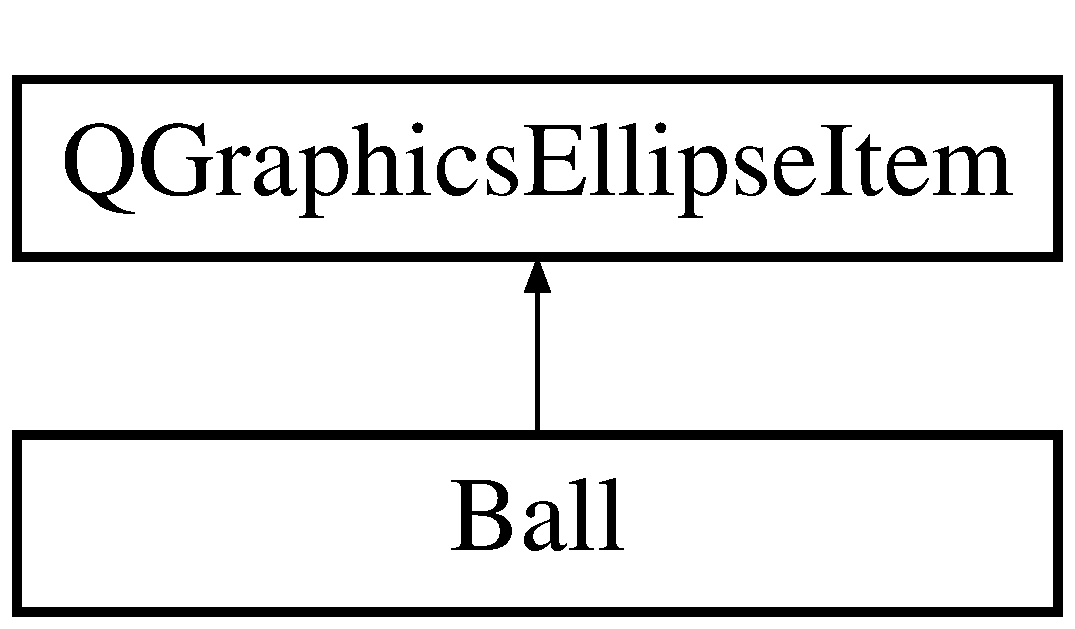
\includegraphics[height=2.000000cm]{classBall}
\end{center}
\end{figure}
\subsection*{Public Member Functions}
\begin{DoxyCompactItemize}
\item 
\hypertarget{classBall_aa7fd02a53e4a659af542ae0a43347eb0}{{\bfseries Ball} (\hyperlink{classBallConfigItem}{Ball\-Config\-Item} $\ast$config)}\label{classBall_aa7fd02a53e4a659af542ae0a43347eb0}

\item 
\hypertarget{classBall_adc25aa6b771ad0bf296d10db4ebcd158}{void {\bfseries advance} (int phase)}\label{classBall_adc25aa6b771ad0bf296d10db4ebcd158}

\item 
\hypertarget{classBall_ac98f05d69458a27ba3b98edb07c3a2fa}{Q\-Point\-F {\bfseries get\-Center} () const }\label{classBall_ac98f05d69458a27ba3b98edb07c3a2fa}

\item 
\hypertarget{classBall_a7932545632a5c6faea61336d707a9c5b}{int {\bfseries get\-Radius} () const }\label{classBall_a7932545632a5c6faea61336d707a9c5b}

\item 
\hypertarget{classBall_a4f69330e1f4f6a554cfc9e4cba091440}{Q\-Vector2\-D {\bfseries get\-Velocity} () const }\label{classBall_a4f69330e1f4f6a554cfc9e4cba091440}

\item 
\hypertarget{classBall_aaa7ecfb934f2ace670bdf81eb0bf712e}{void {\bfseries set\-Velocity} (const Q\-Vector2\-D \&new\-Velocity)}\label{classBall_aaa7ecfb934f2ace670bdf81eb0bf712e}

\end{DoxyCompactItemize}


\subsection{Detailed Description}
The \hyperlink{classBall}{Ball} class. 

The documentation for this class was generated from the following files\-:\begin{DoxyCompactItemize}
\item 
ball.\-h\item 
ball.\-cpp\end{DoxyCompactItemize}

\hypertarget{classBallConfigItem}{\section{Ball\-Config\-Item Class Reference}
\label{classBallConfigItem}\index{Ball\-Config\-Item@{Ball\-Config\-Item}}
}


{\ttfamily \#include $<$ballconfigitem.\-h$>$}

Inheritance diagram for Ball\-Config\-Item\-:\begin{figure}[H]
\begin{center}
\leavevmode
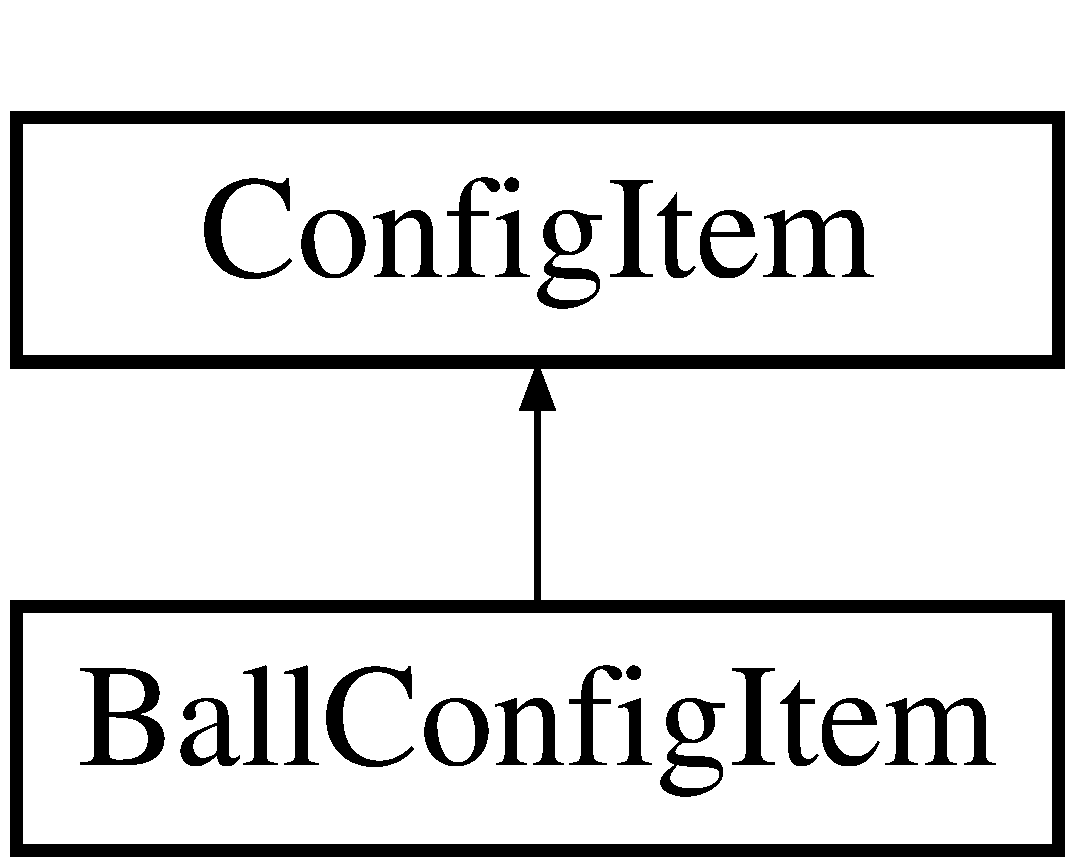
\includegraphics[height=2.000000cm]{classBallConfigItem}
\end{center}
\end{figure}
\subsection*{Public Member Functions}
\begin{DoxyCompactItemize}
\item 
\hypertarget{classBallConfigItem_ae3b96332ceedd324cca9e103f49c02e0}{bool \hyperlink{classBallConfigItem_ae3b96332ceedd324cca9e103f49c02e0}{validate} (int height, int width) const }\label{classBallConfigItem_ae3b96332ceedd324cca9e103f49c02e0}

\begin{DoxyCompactList}\small\item\em validate \end{DoxyCompactList}\item 
\hypertarget{classBallConfigItem_af6ac195294f3ec979966d1bb3630244e}{Item {\bfseries get\-Item\-Type} () const }\label{classBallConfigItem_af6ac195294f3ec979966d1bb3630244e}

\item 
\hypertarget{classBallConfigItem_a72d0624866b2ba494dc96c0a9c900a34}{void {\bfseries add\-Parameter} (std\-::string name, double value)}\label{classBallConfigItem_a72d0624866b2ba494dc96c0a9c900a34}

\item 
Q\-Point\-F \hyperlink{classBallConfigItem_a14b2c2bfde025cb9b5ed4616aa7ef652}{get\-Coordinates} () const 
\item 
\hypertarget{classBallConfigItem_a5bb1e113d6f47c03b68803f37a136b4a}{void {\bfseries set\-Coordinate} (Q\-Point\-F const \&ncoor)}\label{classBallConfigItem_a5bb1e113d6f47c03b68803f37a136b4a}

\item 
\hypertarget{classBallConfigItem_a334cb9d9683fb1631a252fafbb045e4d}{void {\bfseries set\-X\-Coordinate} (int)}\label{classBallConfigItem_a334cb9d9683fb1631a252fafbb045e4d}

\item 
\hypertarget{classBallConfigItem_a044e72a6289b872a3bc83f76332027f4}{void {\bfseries set\-Y\-Coordinate} (int)}\label{classBallConfigItem_a044e72a6289b872a3bc83f76332027f4}

\item 
\hypertarget{classBallConfigItem_a9ccb7fcbe037c7e7fa743b10b7b8dfac}{int {\bfseries get\-Radius} () const }\label{classBallConfigItem_a9ccb7fcbe037c7e7fa743b10b7b8dfac}

\item 
\hypertarget{classBallConfigItem_a43926c30079eecf2ede3e1ad2d72259e}{void {\bfseries set\-Radius} (int)}\label{classBallConfigItem_a43926c30079eecf2ede3e1ad2d72259e}

\item 
Q\-Vector2\-D \hyperlink{classBallConfigItem_a8904b6b51a76adce2ec0f3bccbcb5a77}{get\-Velocity} () const 
\item 
\hypertarget{classBallConfigItem_afcc9b01b66ec2ff098e632f1f65b46e8}{void {\bfseries set\-Velocity} (float, float)}\label{classBallConfigItem_afcc9b01b66ec2ff098e632f1f65b46e8}

\item 
\hypertarget{classBallConfigItem_ab4ead3248eaf21df972cffecc1f8d84f}{void {\bfseries set\-X\-Velocity} (float)}\label{classBallConfigItem_ab4ead3248eaf21df972cffecc1f8d84f}

\item 
\hypertarget{classBallConfigItem_a5ac1e20cc83ed6071a70ae4df7fe38ec}{void {\bfseries set\-Y\-Velocity} (float)}\label{classBallConfigItem_a5ac1e20cc83ed6071a70ae4df7fe38ec}

\item 
\hypertarget{classBallConfigItem_ad33c2bd7a2d9f7279a31e63fa3352ab8}{Q\-Color {\bfseries get\-Color} () const }\label{classBallConfigItem_ad33c2bd7a2d9f7279a31e63fa3352ab8}

\item 
\hypertarget{classBallConfigItem_a43ff7257f2c6836b90a5aff2afb66304}{void {\bfseries set\-Hue} (float)}\label{classBallConfigItem_a43ff7257f2c6836b90a5aff2afb66304}

\end{DoxyCompactItemize}


\subsection{Detailed Description}
The config item for a ball. Reworked to interface better with a Q\-Graphics\-Item. 

\subsection{Member Function Documentation}
\hypertarget{classBallConfigItem_a14b2c2bfde025cb9b5ed4616aa7ef652}{\index{Ball\-Config\-Item@{Ball\-Config\-Item}!get\-Coordinates@{get\-Coordinates}}
\index{get\-Coordinates@{get\-Coordinates}!BallConfigItem@{Ball\-Config\-Item}}
\subsubsection[{get\-Coordinates}]{\setlength{\rightskip}{0pt plus 5cm}Q\-Point\-F Ball\-Config\-Item\-::get\-Coordinates (
\begin{DoxyParamCaption}
{}
\end{DoxyParamCaption}
) const\hspace{0.3cm}{\ttfamily [inline]}}}\label{classBallConfigItem_a14b2c2bfde025cb9b5ed4616aa7ef652}
Setters and getters for the coordinates. \hypertarget{classBallConfigItem_a8904b6b51a76adce2ec0f3bccbcb5a77}{\index{Ball\-Config\-Item@{Ball\-Config\-Item}!get\-Velocity@{get\-Velocity}}
\index{get\-Velocity@{get\-Velocity}!BallConfigItem@{Ball\-Config\-Item}}
\subsubsection[{get\-Velocity}]{\setlength{\rightskip}{0pt plus 5cm}Q\-Vector2\-D Ball\-Config\-Item\-::get\-Velocity (
\begin{DoxyParamCaption}
{}
\end{DoxyParamCaption}
) const\hspace{0.3cm}{\ttfamily [inline]}}}\label{classBallConfigItem_a8904b6b51a76adce2ec0f3bccbcb5a77}
Methods to care about the velocity. 

The documentation for this class was generated from the following files\-:\begin{DoxyCompactItemize}
\item 
ballconfigitem.\-h\item 
ballconfigitem.\-cpp\end{DoxyCompactItemize}

\hypertarget{classBallLostEvent}{\section{Ball\-Lost\-Event Class Reference}
\label{classBallLostEvent}\index{Ball\-Lost\-Event@{Ball\-Lost\-Event}}
}


The ball was lost at the bottom.  




{\ttfamily \#include $<$Events.\-h$>$}

Inheritance diagram for Ball\-Lost\-Event\-:\begin{figure}[H]
\begin{center}
\leavevmode
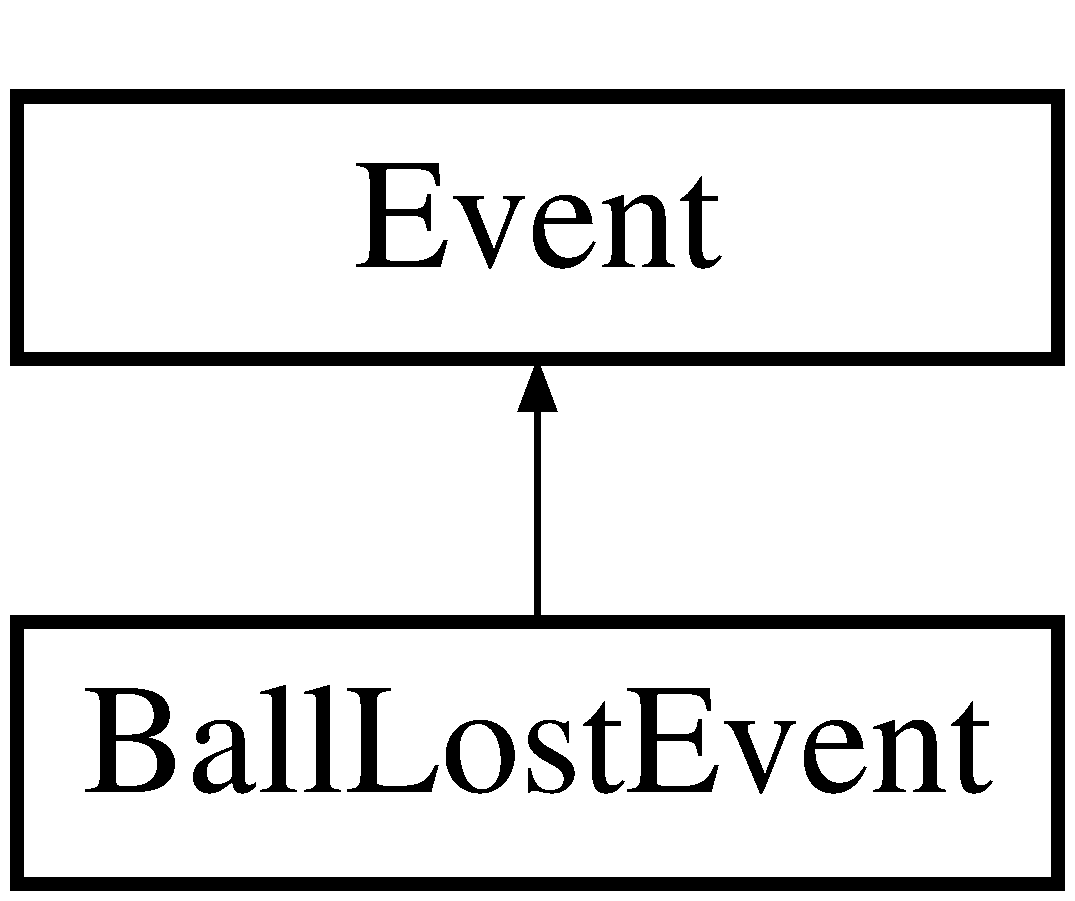
\includegraphics[height=2.000000cm]{classBallLostEvent}
\end{center}
\end{figure}
\subsection*{Additional Inherited Members}


\subsection{Detailed Description}
The ball was lost at the bottom. 

The documentation for this class was generated from the following file\-:\begin{DoxyCompactItemize}
\item 
Events.\-h\end{DoxyCompactItemize}

\hypertarget{classBlock}{\section{Block Class Reference}
\label{classBlock}\index{Block@{Block}}
}


The \hyperlink{classBlock}{Block} class.  




{\ttfamily \#include $<$block.\-h$>$}

Inheritance diagram for Block\-:\begin{figure}[H]
\begin{center}
\leavevmode
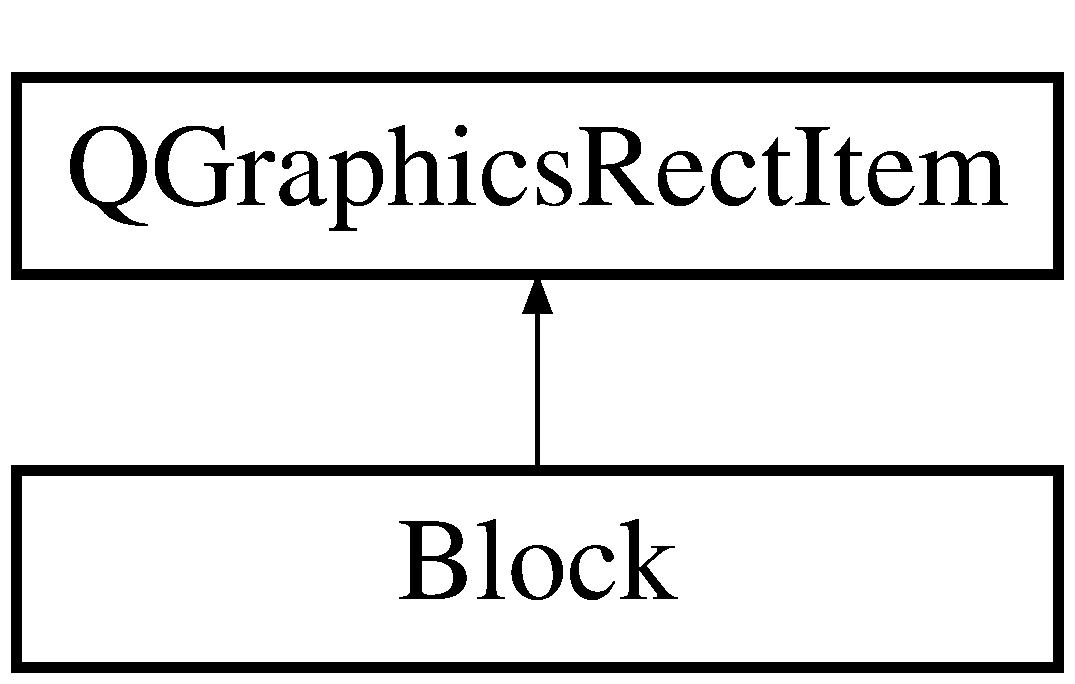
\includegraphics[height=2.000000cm]{classBlock}
\end{center}
\end{figure}
\subsection*{Public Member Functions}
\begin{DoxyCompactItemize}
\item 
\hypertarget{classBlock_af21c73da78352f1ec4d36b9725533b8f}{{\bfseries Block} (\hyperlink{classBlockConfigItem}{Block\-Config\-Item} $\ast$config)}\label{classBlock_af21c73da78352f1ec4d36b9725533b8f}

\item 
\hypertarget{classBlock_ae0ae7cd39933b1b5a856473c3ed0c8bc}{void {\bfseries advance} (int phase)}\label{classBlock_ae0ae7cd39933b1b5a856473c3ed0c8bc}

\item 
\hypertarget{classBlock_ab12fdff5173a545366df5e01e91588f1}{Q\-Point\-F {\bfseries get\-Position} () const }\label{classBlock_ab12fdff5173a545366df5e01e91588f1}

\item 
\hypertarget{classBlock_a4a30ffe76ac7d5002d1f6a600bf8635c}{int {\bfseries get\-Lives} () const }\label{classBlock_a4a30ffe76ac7d5002d1f6a600bf8635c}

\item 
\hypertarget{classBlock_a374a82896efe68591942d76c4209605a}{void {\bfseries decrement\-Lives} ()}\label{classBlock_a374a82896efe68591942d76c4209605a}

\end{DoxyCompactItemize}


\subsection{Detailed Description}
The \hyperlink{classBlock}{Block} class. 

The documentation for this class was generated from the following files\-:\begin{DoxyCompactItemize}
\item 
block.\-h\item 
block.\-cpp\end{DoxyCompactItemize}

\hypertarget{classBlockConfigItem}{\section{Block\-Config\-Item Class Reference}
\label{classBlockConfigItem}\index{Block\-Config\-Item@{Block\-Config\-Item}}
}
Inheritance diagram for Block\-Config\-Item\-:\begin{figure}[H]
\begin{center}
\leavevmode
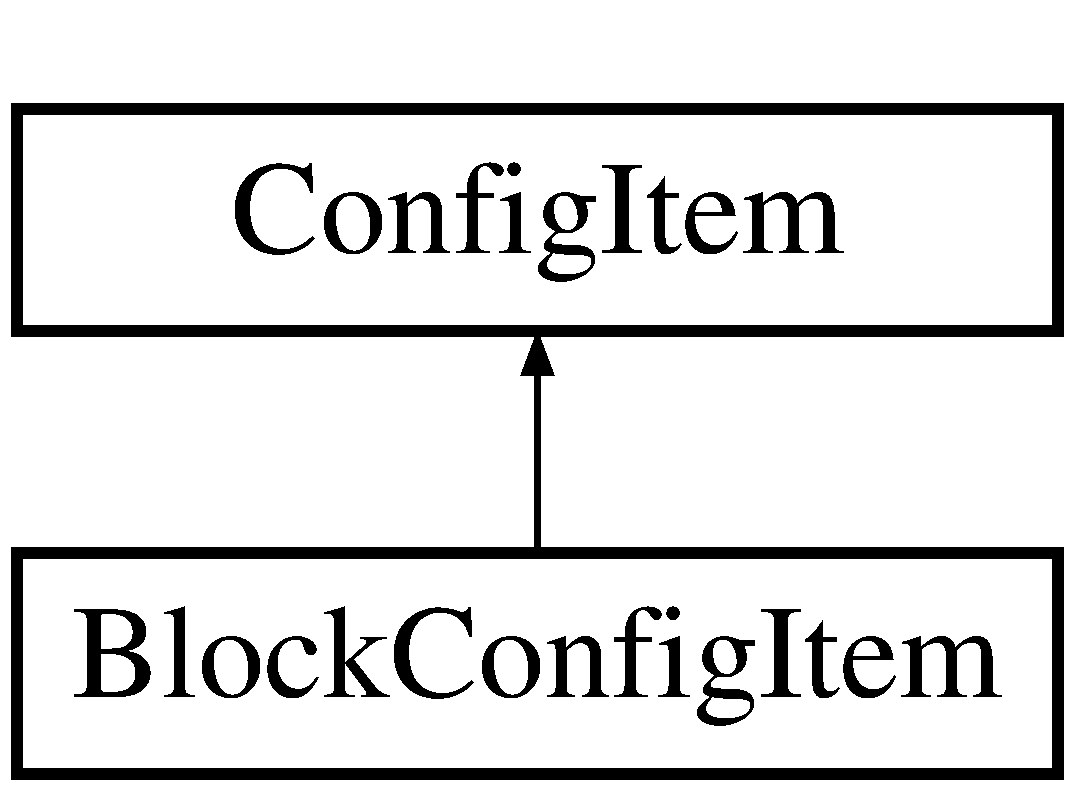
\includegraphics[height=2.000000cm]{classBlockConfigItem}
\end{center}
\end{figure}
\subsection*{Public Member Functions}
\begin{DoxyCompactItemize}
\item 
\hypertarget{classBlockConfigItem_ae60a46647e2c32ef3fe61d845fe20653}{bool \hyperlink{classBlockConfigItem_ae60a46647e2c32ef3fe61d845fe20653}{validate} (int height, int width) const }\label{classBlockConfigItem_ae60a46647e2c32ef3fe61d845fe20653}

\begin{DoxyCompactList}\small\item\em validate \end{DoxyCompactList}\item 
\hypertarget{classBlockConfigItem_a0c7ac57d0f2d42bef3ba48f0241599cb}{Item {\bfseries get\-Item\-Type} () const }\label{classBlockConfigItem_a0c7ac57d0f2d42bef3ba48f0241599cb}

\item 
\hypertarget{classBlockConfigItem_a71fb07630e0bac96aaa25bf52896736f}{void {\bfseries add\-Parameter} (std\-::string name, double value)}\label{classBlockConfigItem_a71fb07630e0bac96aaa25bf52896736f}

\item 
\hypertarget{classBlockConfigItem_a13dc8cc072d44c09f0428ef9df72cbb5}{Q\-Rect\-F const {\bfseries get\-Rect} () const }\label{classBlockConfigItem_a13dc8cc072d44c09f0428ef9df72cbb5}

\item 
\hypertarget{classBlockConfigItem_ae33e71a9ba70019636a49329a39fec90}{Q\-Point\-F const {\bfseries get\-Coordinates} () const }\label{classBlockConfigItem_ae33e71a9ba70019636a49329a39fec90}

\item 
\hypertarget{classBlockConfigItem_a62fba644d2219719359eb09ffba10f80}{void {\bfseries set\-X\-Coordinate} (int)}\label{classBlockConfigItem_a62fba644d2219719359eb09ffba10f80}

\item 
\hypertarget{classBlockConfigItem_adcd88548479a1cdb3a5179983c6a35aa}{void {\bfseries set\-Y\-Coordinate} (int)}\label{classBlockConfigItem_adcd88548479a1cdb3a5179983c6a35aa}

\item 
\hypertarget{classBlockConfigItem_aa69e92e67f3d87fa1b8c352a8aa330df}{int {\bfseries get\-Width} () const }\label{classBlockConfigItem_aa69e92e67f3d87fa1b8c352a8aa330df}

\item 
\hypertarget{classBlockConfigItem_a98fbcad50cb8a7bd2e637f139d426d33}{void {\bfseries set\-Width} (int)}\label{classBlockConfigItem_a98fbcad50cb8a7bd2e637f139d426d33}

\item 
\hypertarget{classBlockConfigItem_a216bc2cdf3b351900d7b621250ca803e}{int {\bfseries get\-Height} () const }\label{classBlockConfigItem_a216bc2cdf3b351900d7b621250ca803e}

\item 
\hypertarget{classBlockConfigItem_a70e7d230c8116ae104a21bfaa7007a6f}{void {\bfseries set\-Height} (int)}\label{classBlockConfigItem_a70e7d230c8116ae104a21bfaa7007a6f}

\item 
\hypertarget{classBlockConfigItem_a6970ee35a9fca796deeffa002b7a3efb}{int {\bfseries get\-Lives} () const }\label{classBlockConfigItem_a6970ee35a9fca796deeffa002b7a3efb}

\item 
\hypertarget{classBlockConfigItem_ae359c77e2804984f1a0b6f75643d9257}{void {\bfseries set\-Lives} (int)}\label{classBlockConfigItem_ae359c77e2804984f1a0b6f75643d9257}

\item 
\hypertarget{classBlockConfigItem_ab8892b6722c7201f0a3faad0c1860c9d}{Q\-Color {\bfseries get\-Color} () const }\label{classBlockConfigItem_ab8892b6722c7201f0a3faad0c1860c9d}

\item 
\hypertarget{classBlockConfigItem_aceeb33135f45c110b057359fac7ccab3}{void {\bfseries set\-Hue} (float)}\label{classBlockConfigItem_aceeb33135f45c110b057359fac7ccab3}

\end{DoxyCompactItemize}


The documentation for this class was generated from the following files\-:\begin{DoxyCompactItemize}
\item 
blockconfigitem.\-h\item 
blockconfigitem.\-cpp\end{DoxyCompactItemize}

\hypertarget{classBlockDeletedEvent}{\section{Block\-Deleted\-Event Class Reference}
\label{classBlockDeletedEvent}\index{Block\-Deleted\-Event@{Block\-Deleted\-Event}}
}


Triggered when a block is removed from the scene.  




{\ttfamily \#include $<$Events.\-h$>$}

Inheritance diagram for Block\-Deleted\-Event\-:\begin{figure}[H]
\begin{center}
\leavevmode
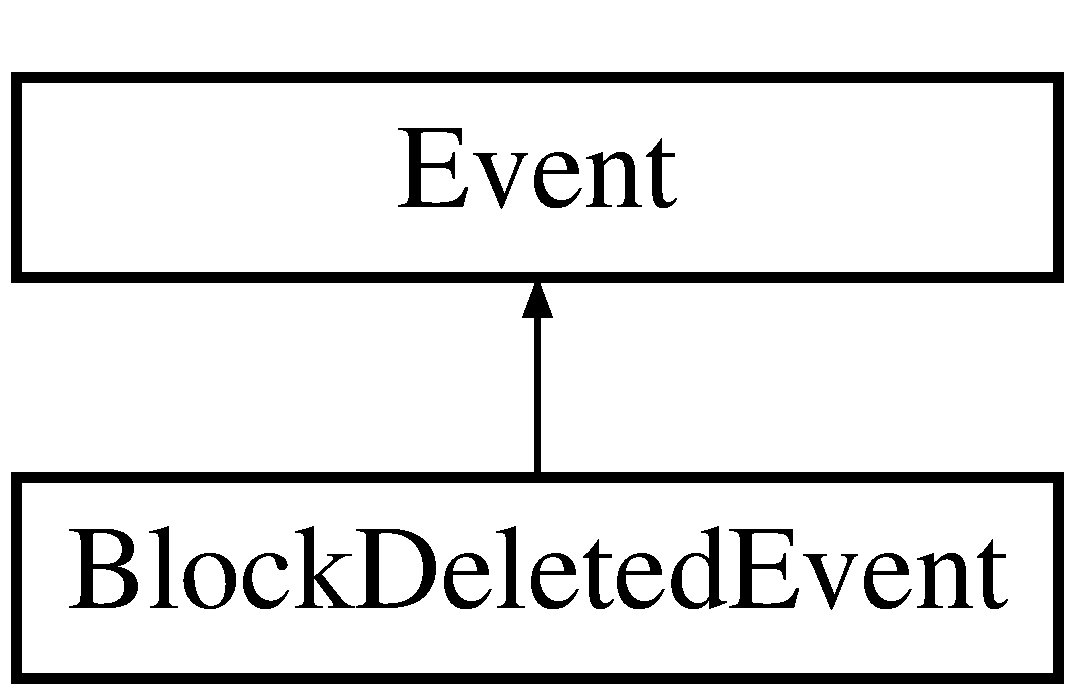
\includegraphics[height=2.000000cm]{classBlockDeletedEvent}
\end{center}
\end{figure}
\subsection*{Additional Inherited Members}


\subsection{Detailed Description}
Triggered when a block is removed from the scene. 

The documentation for this class was generated from the following file\-:\begin{DoxyCompactItemize}
\item 
Events.\-h\end{DoxyCompactItemize}

\hypertarget{classChainOfResponsibility}{\section{Chain\-Of\-Responsibility Class Reference}
\label{classChainOfResponsibility}\index{Chain\-Of\-Responsibility@{Chain\-Of\-Responsibility}}
}


Traverse chain of responsibility and manage it.  




{\ttfamily \#include $<$chainofresponsibility.\-h$>$}

\subsection*{Public Member Functions}
\begin{DoxyCompactItemize}
\item 
void \hyperlink{classChainOfResponsibility_a59e7c6850bbbef64d53043fc78ac8b8b}{add} (\hyperlink{classAbstractResponsibility}{Abstract\-Responsibility} $\ast$)
\item 
void \hyperlink{classChainOfResponsibility_ab452d547a94bb23a0417f81850ca0601}{remove} (\hyperlink{classAbstractResponsibility}{Abstract\-Responsibility} $\ast$)
\item 
void \hyperlink{classChainOfResponsibility_a068f5080af0681aadf0d1a9292b21988}{handle\-Event} (\hyperlink{classEvent}{Event} $\ast$)
\end{DoxyCompactItemize}
\subsection*{Static Public Member Functions}
\begin{DoxyCompactItemize}
\item 
static \hyperlink{classChainOfResponsibility}{Chain\-Of\-Responsibility} \& \hyperlink{classChainOfResponsibility_aeefa4eddd729640133be4c7bcc1a99c8}{get} ()
\end{DoxyCompactItemize}
\subsection*{Protected Member Functions}
\begin{DoxyCompactItemize}
\item 
void \hyperlink{classChainOfResponsibility_acb45d69622de806430f898d5a27145dc}{reset} ()
\end{DoxyCompactItemize}
\subsection*{Friends}
\begin{DoxyCompactItemize}
\item 
\hypertarget{classChainOfResponsibility_ab9aaba231fd11196425e75caf709bfc6}{class {\bfseries Test\-Suite}}\label{classChainOfResponsibility_ab9aaba231fd11196425e75caf709bfc6}

\end{DoxyCompactItemize}


\subsection{Detailed Description}
Traverse chain of responsibility and manage it. 

The central place of the only chain of responsibility in this programm. This class is implemented as Singleton (p. 127 Go\-F-\/book). Adding and removing of participants of the chain of responsibility as well as pushing an event into the chain is simplified by this class. 

\subsection{Member Function Documentation}
\hypertarget{classChainOfResponsibility_a59e7c6850bbbef64d53043fc78ac8b8b}{\index{Chain\-Of\-Responsibility@{Chain\-Of\-Responsibility}!add@{add}}
\index{add@{add}!ChainOfResponsibility@{Chain\-Of\-Responsibility}}
\subsubsection[{add}]{\setlength{\rightskip}{0pt plus 5cm}void Chain\-Of\-Responsibility\-::add (
\begin{DoxyParamCaption}
\item[{{\bf Abstract\-Responsibility} $\ast$}]{n}
\end{DoxyParamCaption}
)}}\label{classChainOfResponsibility_a59e7c6850bbbef64d53043fc78ac8b8b}
Add a member to the chain. \hypertarget{classChainOfResponsibility_aeefa4eddd729640133be4c7bcc1a99c8}{\index{Chain\-Of\-Responsibility@{Chain\-Of\-Responsibility}!get@{get}}
\index{get@{get}!ChainOfResponsibility@{Chain\-Of\-Responsibility}}
\subsubsection[{get}]{\setlength{\rightskip}{0pt plus 5cm}{\bf Chain\-Of\-Responsibility} \& Chain\-Of\-Responsibility\-::get (
\begin{DoxyParamCaption}
{}
\end{DoxyParamCaption}
)\hspace{0.3cm}{\ttfamily [static]}}}\label{classChainOfResponsibility_aeefa4eddd729640133be4c7bcc1a99c8}
Get the only instance of the chain of responbility. \hypertarget{classChainOfResponsibility_a068f5080af0681aadf0d1a9292b21988}{\index{Chain\-Of\-Responsibility@{Chain\-Of\-Responsibility}!handle\-Event@{handle\-Event}}
\index{handle\-Event@{handle\-Event}!ChainOfResponsibility@{Chain\-Of\-Responsibility}}
\subsubsection[{handle\-Event}]{\setlength{\rightskip}{0pt plus 5cm}void Chain\-Of\-Responsibility\-::handle\-Event (
\begin{DoxyParamCaption}
\item[{{\bf Event} $\ast$}]{event}
\end{DoxyParamCaption}
)}}\label{classChainOfResponsibility_a068f5080af0681aadf0d1a9292b21988}
Propagate an event through the chain of responsibility. \hypertarget{classChainOfResponsibility_ab452d547a94bb23a0417f81850ca0601}{\index{Chain\-Of\-Responsibility@{Chain\-Of\-Responsibility}!remove@{remove}}
\index{remove@{remove}!ChainOfResponsibility@{Chain\-Of\-Responsibility}}
\subsubsection[{remove}]{\setlength{\rightskip}{0pt plus 5cm}void Chain\-Of\-Responsibility\-::remove (
\begin{DoxyParamCaption}
\item[{{\bf Abstract\-Responsibility} $\ast$}]{item}
\end{DoxyParamCaption}
)}}\label{classChainOfResponsibility_ab452d547a94bb23a0417f81850ca0601}
Remove the member given. \hypertarget{classChainOfResponsibility_acb45d69622de806430f898d5a27145dc}{\index{Chain\-Of\-Responsibility@{Chain\-Of\-Responsibility}!reset@{reset}}
\index{reset@{reset}!ChainOfResponsibility@{Chain\-Of\-Responsibility}}
\subsubsection[{reset}]{\setlength{\rightskip}{0pt plus 5cm}void Chain\-Of\-Responsibility\-::reset (
\begin{DoxyParamCaption}
{}
\end{DoxyParamCaption}
)\hspace{0.3cm}{\ttfamily [protected]}}}\label{classChainOfResponsibility_acb45d69622de806430f898d5a27145dc}
Needed for testing only. 

The documentation for this class was generated from the following files\-:\begin{DoxyCompactItemize}
\item 
chainofresponsibility.\-h\item 
chainofresponsibility.\-cpp\end{DoxyCompactItemize}

\hypertarget{classConfig}{\section{Config Class Reference}
\label{classConfig}\index{Config@{Config}}
}
\subsection*{Public Member Functions}
\begin{DoxyCompactItemize}
\item 
\hypertarget{classConfig_abd0c571c116924871e30444b192b792a}{\hyperlink{classConfig_abd0c571c116924871e30444b192b792a}{Config} ()}\label{classConfig_abd0c571c116924871e30444b192b792a}

\begin{DoxyCompactList}\small\item\em \hyperlink{classConfig_abd0c571c116924871e30444b192b792a}{Config\-::\-Config} Construct a config and read in from the default location. \end{DoxyCompactList}\item 
\hyperlink{classConfig_a543dce59b66475c5108088ee4ce1cdfc}{$\sim$\-Config} ()
\item 
\hypertarget{classConfig_ae18d6754d79fb80ee0cd21214803bf67}{size\-\_\-t {\bfseries size} () const }\label{classConfig_ae18d6754d79fb80ee0cd21214803bf67}

\item 
\hypertarget{classConfig_ae215a8a66df0fde217ca911553c563a1}{\hyperlink{classConfigItem}{Config\-Item} $\ast$ {\bfseries operator\mbox{[}$\,$\mbox{]}} (int i)}\label{classConfig_ae215a8a66df0fde217ca911553c563a1}

\item 
\hypertarget{classConfig_a6b856d23ba155616807e8aba36bdf54f}{int {\bfseries get\-Width} () const }\label{classConfig_a6b856d23ba155616807e8aba36bdf54f}

\item 
\hypertarget{classConfig_a51ba2044146393de06fe2139a04fa899}{int {\bfseries get\-Height} () const }\label{classConfig_a51ba2044146393de06fe2139a04fa899}

\end{DoxyCompactItemize}


\subsection{Constructor \& Destructor Documentation}
\hypertarget{classConfig_a543dce59b66475c5108088ee4ce1cdfc}{\index{Config@{Config}!$\sim$\-Config@{$\sim$\-Config}}
\index{$\sim$\-Config@{$\sim$\-Config}!Config@{Config}}
\subsubsection[{$\sim$\-Config}]{\setlength{\rightskip}{0pt plus 5cm}Config\-::$\sim$\-Config (
\begin{DoxyParamCaption}
{}
\end{DoxyParamCaption}
)}}\label{classConfig_a543dce59b66475c5108088ee4ce1cdfc}
Delete the config items on config deletion. 

The documentation for this class was generated from the following files\-:\begin{DoxyCompactItemize}
\item 
config.\-h\item 
config.\-cpp\end{DoxyCompactItemize}

\hypertarget{classConfigItem}{\section{Config\-Item Class Reference}
\label{classConfigItem}\index{Config\-Item@{Config\-Item}}
}
Inheritance diagram for Config\-Item\-:\begin{figure}[H]
\begin{center}
\leavevmode
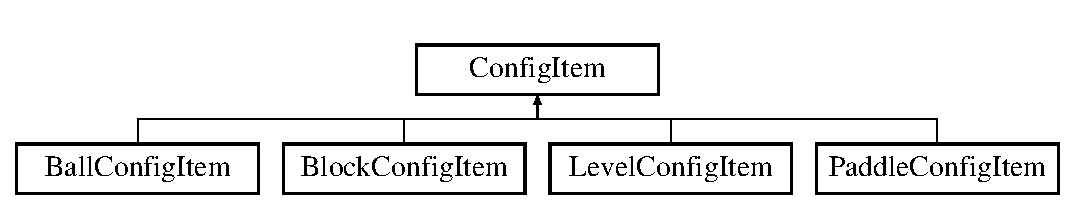
\includegraphics[height=2.000000cm]{classConfigItem}
\end{center}
\end{figure}
\subsection*{Public Member Functions}
\begin{DoxyCompactItemize}
\item 
\hypertarget{classConfigItem_a0ffeae3ab9688202ad167e15ccb3be6d}{virtual bool \hyperlink{classConfigItem_a0ffeae3ab9688202ad167e15ccb3be6d}{validate} (int height, int width) const =0}\label{classConfigItem_a0ffeae3ab9688202ad167e15ccb3be6d}

\begin{DoxyCompactList}\small\item\em validate \end{DoxyCompactList}\item 
\hypertarget{classConfigItem_afe4d414a6a586a8867dd774caf0a4e52}{virtual Item {\bfseries get\-Item\-Type} () const =0}\label{classConfigItem_afe4d414a6a586a8867dd774caf0a4e52}

\item 
\hypertarget{classConfigItem_a5c3b2b8e0e88dffaf3874143a9876773}{virtual void {\bfseries add\-Parameter} (std\-::string name, double value)=0}\label{classConfigItem_a5c3b2b8e0e88dffaf3874143a9876773}

\item 
virtual \hyperlink{classConfigItem_a609948948b73783000be262ed09ffc6e}{$\sim$\-Config\-Item} ()
\end{DoxyCompactItemize}


\subsection{Constructor \& Destructor Documentation}
\hypertarget{classConfigItem_a609948948b73783000be262ed09ffc6e}{\index{Config\-Item@{Config\-Item}!$\sim$\-Config\-Item@{$\sim$\-Config\-Item}}
\index{$\sim$\-Config\-Item@{$\sim$\-Config\-Item}!ConfigItem@{Config\-Item}}
\subsubsection[{$\sim$\-Config\-Item}]{\setlength{\rightskip}{0pt plus 5cm}virtual Config\-Item\-::$\sim$\-Config\-Item (
\begin{DoxyParamCaption}
{}
\end{DoxyParamCaption}
)\hspace{0.3cm}{\ttfamily [inline]}, {\ttfamily [virtual]}}}\label{classConfigItem_a609948948b73783000be262ed09ffc6e}
Add virtual destructor, to make sure all derived classes' objects are destroyed correctly. 

The documentation for this class was generated from the following file\-:\begin{DoxyCompactItemize}
\item 
configitem.\-h\end{DoxyCompactItemize}

\hypertarget{classDialog}{\section{Dialog Class Reference}
\label{classDialog}\index{Dialog@{Dialog}}
}
Inheritance diagram for Dialog\-:\begin{figure}[H]
\begin{center}
\leavevmode
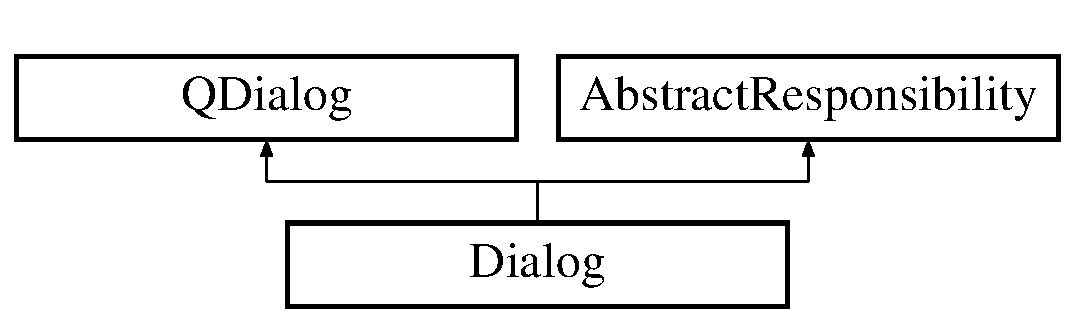
\includegraphics[height=2.000000cm]{classDialog}
\end{center}
\end{figure}
\subsection*{Public Slots}
\begin{DoxyCompactItemize}
\item 
\hypertarget{classDialog_a8bc4fe3b0cc12033369b49eab8751e14}{void {\bfseries next\-Frame} ()}\label{classDialog_a8bc4fe3b0cc12033369b49eab8751e14}

\end{DoxyCompactItemize}
\subsection*{Public Member Functions}
\begin{DoxyCompactItemize}
\item 
\hypertarget{classDialog_a92143e1be7913dd7cdb93a3abfc53ebc}{{\bfseries Dialog} (\hyperlink{classConfig}{Config} $\ast$config, Q\-Widget $\ast$parent=0)}\label{classDialog_a92143e1be7913dd7cdb93a3abfc53ebc}

\item 
\hyperlink{classDialog_a2a1fe6ef28513eed13bfcd3a4da83ccb}{$\sim$\-Dialog} ()
\item 
void \hyperlink{classDialog_a95aaa4d78bda5c07650d383d3c5292ac}{mouse\-Press\-Event} (Q\-Mouse\-Event $\ast$event)
\begin{DoxyCompactList}\small\item\em \hyperlink{classDialog_a95aaa4d78bda5c07650d383d3c5292ac}{Dialog\-::mouse\-Press\-Event} stores the. \end{DoxyCompactList}\item 
void \hyperlink{classDialog_a97894cd3d240b62d9da4f915b9e16a12}{key\-Press\-Event} (Q\-Key\-Event $\ast$)
\item 
void \hyperlink{classDialog_a64bf1a64d37efa953896fbc106f55a56}{handle\-Event} (\hyperlink{classEvent}{Event} $\ast$)
\item 
void \hyperlink{classDialog_ae1dd568c8ea45c8aa7782a5de28846ea}{start\-Timer} ()
\item 
void \hyperlink{classDialog_accd61d9aca9f76417c2129c04d0e7dcf}{stop\-Timer} ()
\end{DoxyCompactItemize}
\subsection*{Additional Inherited Members}


\subsection{Constructor \& Destructor Documentation}
\hypertarget{classDialog_a2a1fe6ef28513eed13bfcd3a4da83ccb}{\index{Dialog@{Dialog}!$\sim$\-Dialog@{$\sim$\-Dialog}}
\index{$\sim$\-Dialog@{$\sim$\-Dialog}!Dialog@{Dialog}}
\subsubsection[{$\sim$\-Dialog}]{\setlength{\rightskip}{0pt plus 5cm}Dialog\-::$\sim$\-Dialog (
\begin{DoxyParamCaption}
{}
\end{DoxyParamCaption}
)}}\label{classDialog_a2a1fe6ef28513eed13bfcd3a4da83ccb}
Destroy the object, freeing all memory. 

\subsection{Member Function Documentation}
\hypertarget{classDialog_a64bf1a64d37efa953896fbc106f55a56}{\index{Dialog@{Dialog}!handle\-Event@{handle\-Event}}
\index{handle\-Event@{handle\-Event}!Dialog@{Dialog}}
\subsubsection[{handle\-Event}]{\setlength{\rightskip}{0pt plus 5cm}void Dialog\-::handle\-Event (
\begin{DoxyParamCaption}
\item[{{\bf Event} $\ast$}]{event}
\end{DoxyParamCaption}
)\hspace{0.3cm}{\ttfamily [virtual]}}}\label{classDialog_a64bf1a64d37efa953896fbc106f55a56}
Handle the key presses for the dialog window, i.\-e., act on Q to quit. 

Reimplemented from \hyperlink{classAbstractResponsibility_a14d885884ae4841dbe7c5824b986f2c9}{Abstract\-Responsibility}.

\hypertarget{classDialog_a97894cd3d240b62d9da4f915b9e16a12}{\index{Dialog@{Dialog}!key\-Press\-Event@{key\-Press\-Event}}
\index{key\-Press\-Event@{key\-Press\-Event}!Dialog@{Dialog}}
\subsubsection[{key\-Press\-Event}]{\setlength{\rightskip}{0pt plus 5cm}void Dialog\-::key\-Press\-Event (
\begin{DoxyParamCaption}
\item[{Q\-Key\-Event $\ast$}]{event}
\end{DoxyParamCaption}
)}}\label{classDialog_a97894cd3d240b62d9da4f915b9e16a12}
Start the chain of responsibility for key presses by overloading the method. \hypertarget{classDialog_a95aaa4d78bda5c07650d383d3c5292ac}{\index{Dialog@{Dialog}!mouse\-Press\-Event@{mouse\-Press\-Event}}
\index{mouse\-Press\-Event@{mouse\-Press\-Event}!Dialog@{Dialog}}
\subsubsection[{mouse\-Press\-Event}]{\setlength{\rightskip}{0pt plus 5cm}void Dialog\-::mouse\-Press\-Event (
\begin{DoxyParamCaption}
\item[{Q\-Mouse\-Event $\ast$}]{event}
\end{DoxyParamCaption}
)}}\label{classDialog_a95aaa4d78bda5c07650d383d3c5292ac}


\hyperlink{classDialog_a95aaa4d78bda5c07650d383d3c5292ac}{Dialog\-::mouse\-Press\-Event} stores the. 

Handle mouse clicks.


\begin{DoxyParams}{Parameters}
{\em event} & \\
\hline
\end{DoxyParams}
\hypertarget{classDialog_ae1dd568c8ea45c8aa7782a5de28846ea}{\index{Dialog@{Dialog}!start\-Timer@{start\-Timer}}
\index{start\-Timer@{start\-Timer}!Dialog@{Dialog}}
\subsubsection[{start\-Timer}]{\setlength{\rightskip}{0pt plus 5cm}void Dialog\-::start\-Timer (
\begin{DoxyParamCaption}
{}
\end{DoxyParamCaption}
)}}\label{classDialog_ae1dd568c8ea45c8aa7782a5de28846ea}
(Re-\/)Start the timer. \hypertarget{classDialog_accd61d9aca9f76417c2129c04d0e7dcf}{\index{Dialog@{Dialog}!stop\-Timer@{stop\-Timer}}
\index{stop\-Timer@{stop\-Timer}!Dialog@{Dialog}}
\subsubsection[{stop\-Timer}]{\setlength{\rightskip}{0pt plus 5cm}void Dialog\-::stop\-Timer (
\begin{DoxyParamCaption}
{}
\end{DoxyParamCaption}
)}}\label{classDialog_accd61d9aca9f76417c2129c04d0e7dcf}
Stop the timer. 

The documentation for this class was generated from the following files\-:\begin{DoxyCompactItemize}
\item 
dialog.\-h\item 
dialog.\-cpp\end{DoxyCompactItemize}

\hypertarget{classUi_1_1Dialog}{\section{Ui\-:\-:Dialog Class Reference}
\label{classUi_1_1Dialog}\index{Ui\-::\-Dialog@{Ui\-::\-Dialog}}
}
Inheritance diagram for Ui\-:\-:Dialog\-:\begin{figure}[H]
\begin{center}
\leavevmode
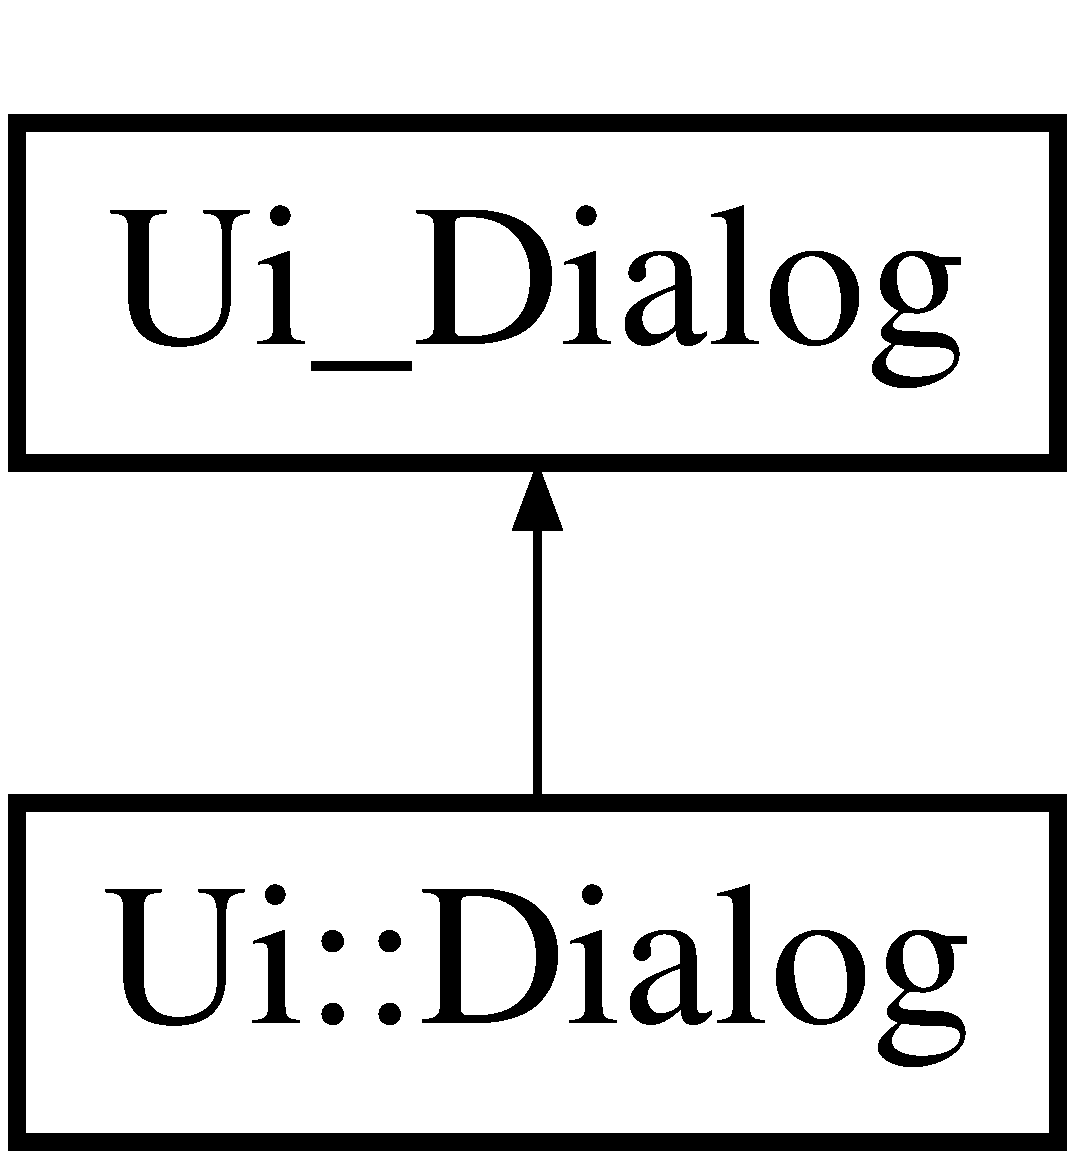
\includegraphics[height=2.000000cm]{classUi_1_1Dialog}
\end{center}
\end{figure}
\subsection*{Additional Inherited Members}


The documentation for this class was generated from the following file\-:\begin{DoxyCompactItemize}
\item 
ui\-\_\-dialog.\-h\end{DoxyCompactItemize}

\hypertarget{classEvent}{\section{Event Class Reference}
\label{classEvent}\index{Event@{Event}}
}


The base structure for all events.  




{\ttfamily \#include $<$Events.\-h$>$}

Inheritance diagram for Event\-:\begin{figure}[H]
\begin{center}
\leavevmode
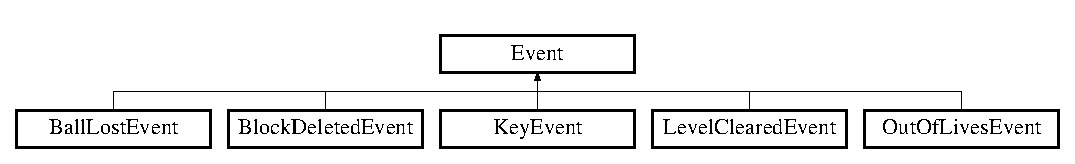
\includegraphics[height=1.750000cm]{classEvent}
\end{center}
\end{figure}
\subsection*{Public Member Functions}
\begin{DoxyCompactItemize}
\item 
virtual \hyperlink{classEvent_ab864fd85c758006c42cd7a1b3369b483}{$\sim$\-Event} ()
\end{DoxyCompactItemize}


\subsection{Detailed Description}
The base structure for all events. 

\subsection{Constructor \& Destructor Documentation}
\hypertarget{classEvent_ab864fd85c758006c42cd7a1b3369b483}{\index{Event@{Event}!$\sim$\-Event@{$\sim$\-Event}}
\index{$\sim$\-Event@{$\sim$\-Event}!Event@{Event}}
\subsubsection[{$\sim$\-Event}]{\setlength{\rightskip}{0pt plus 5cm}virtual Event\-::$\sim$\-Event (
\begin{DoxyParamCaption}
{}
\end{DoxyParamCaption}
)\hspace{0.3cm}{\ttfamily [inline]}, {\ttfamily [virtual]}}}\label{classEvent_ab864fd85c758006c42cd7a1b3369b483}
Ensure the class polymorphic, so that dynamic\-\_\-cast is possible. 

The documentation for this class was generated from the following file\-:\begin{DoxyCompactItemize}
\item 
Events.\-h\end{DoxyCompactItemize}

\hypertarget{classUi_1_1helpDialog}{\section{Ui\-:\-:help\-Dialog Class Reference}
\label{classUi_1_1helpDialog}\index{Ui\-::help\-Dialog@{Ui\-::help\-Dialog}}
}
Inheritance diagram for Ui\-:\-:help\-Dialog\-:\begin{figure}[H]
\begin{center}
\leavevmode
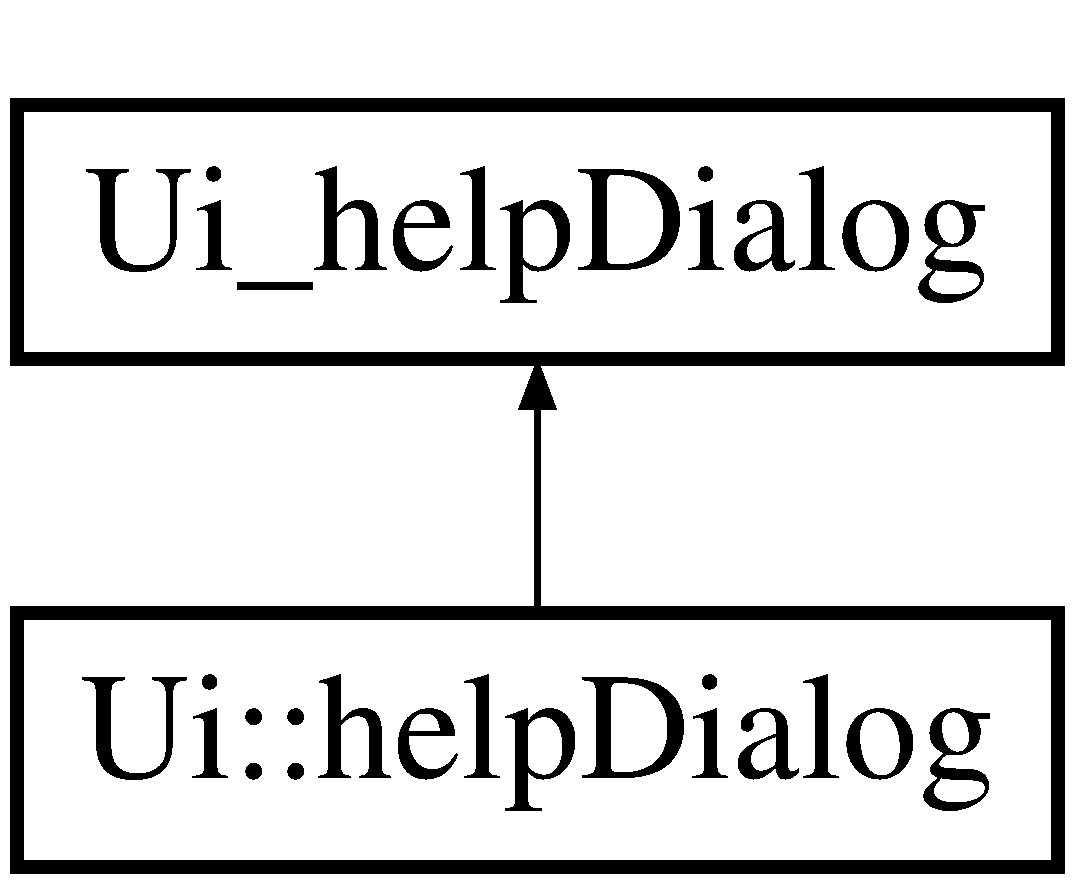
\includegraphics[height=2.000000cm]{classUi_1_1helpDialog}
\end{center}
\end{figure}
\subsection*{Additional Inherited Members}


The documentation for this class was generated from the following file\-:\begin{DoxyCompactItemize}
\item 
ui\-\_\-helpdialog.\-h\end{DoxyCompactItemize}

\hypertarget{classHelpDialogManager}{\section{Help\-Dialog\-Manager Class Reference}
\label{classHelpDialogManager}\index{Help\-Dialog\-Manager@{Help\-Dialog\-Manager}}
}


Display a window with a help text.  




{\ttfamily \#include $<$helpdialogmanager.\-h$>$}

Inheritance diagram for Help\-Dialog\-Manager\-:\begin{figure}[H]
\begin{center}
\leavevmode
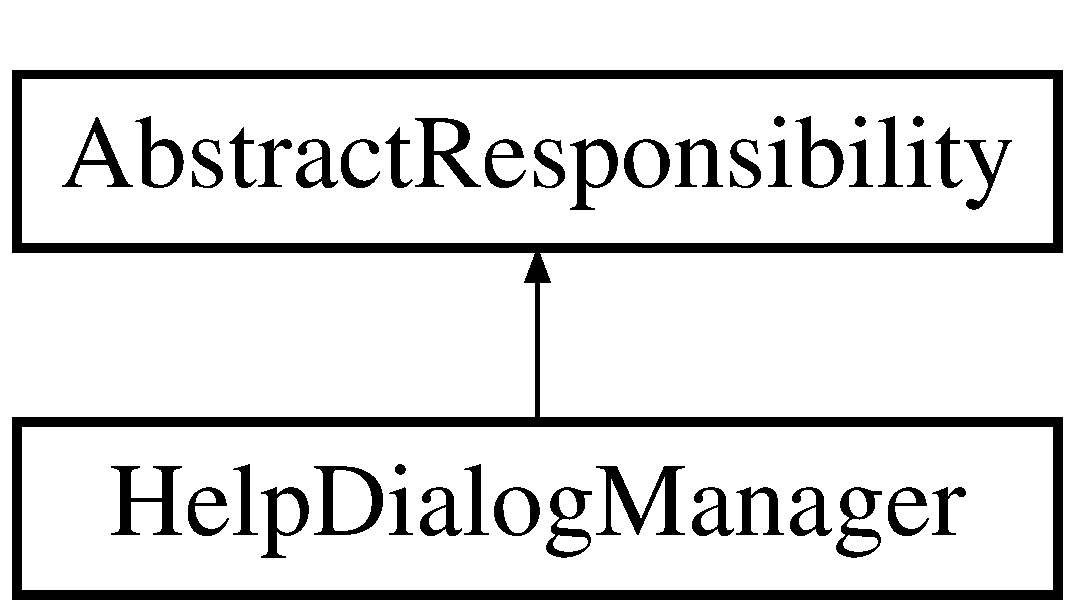
\includegraphics[height=2.000000cm]{classHelpDialogManager}
\end{center}
\end{figure}
\subsection*{Public Member Functions}
\begin{DoxyCompactItemize}
\item 
\hyperlink{classHelpDialogManager_a49833ac06771933b331799ee2ce42dc7}{Help\-Dialog\-Manager} (\hyperlink{classDialog}{Dialog} $\ast$par)
\item 
void \hyperlink{classHelpDialogManager_a5f4d590400c9dc4c3120f8d15ce6b977}{handle\-Event} (\hyperlink{classEvent}{Event} $\ast$)
\end{DoxyCompactItemize}
\subsection*{Additional Inherited Members}


\subsection{Detailed Description}
Display a window with a help text. 

Manage opening a help dialog. The manager waits for key presses of h and ? to display a help window. 

\subsection{Constructor \& Destructor Documentation}
\hypertarget{classHelpDialogManager_a49833ac06771933b331799ee2ce42dc7}{\index{Help\-Dialog\-Manager@{Help\-Dialog\-Manager}!Help\-Dialog\-Manager@{Help\-Dialog\-Manager}}
\index{Help\-Dialog\-Manager@{Help\-Dialog\-Manager}!HelpDialogManager@{Help\-Dialog\-Manager}}
\subsubsection[{Help\-Dialog\-Manager}]{\setlength{\rightskip}{0pt plus 5cm}Help\-Dialog\-Manager\-::\-Help\-Dialog\-Manager (
\begin{DoxyParamCaption}
\item[{{\bf Dialog} $\ast$}]{par}
\end{DoxyParamCaption}
)}}\label{classHelpDialogManager_a49833ac06771933b331799ee2ce42dc7}
Hook ourself into the chain of responsibility, to watch out for help key presses. 

\subsection{Member Function Documentation}
\hypertarget{classHelpDialogManager_a5f4d590400c9dc4c3120f8d15ce6b977}{\index{Help\-Dialog\-Manager@{Help\-Dialog\-Manager}!handle\-Event@{handle\-Event}}
\index{handle\-Event@{handle\-Event}!HelpDialogManager@{Help\-Dialog\-Manager}}
\subsubsection[{handle\-Event}]{\setlength{\rightskip}{0pt plus 5cm}void Help\-Dialog\-Manager\-::handle\-Event (
\begin{DoxyParamCaption}
\item[{{\bf Event} $\ast$}]{key}
\end{DoxyParamCaption}
)\hspace{0.3cm}{\ttfamily [virtual]}}}\label{classHelpDialogManager_a5f4d590400c9dc4c3120f8d15ce6b977}
Handle presses of h and ? keys. 

Reimplemented from \hyperlink{classAbstractResponsibility_a14d885884ae4841dbe7c5824b986f2c9}{Abstract\-Responsibility}.



The documentation for this class was generated from the following files\-:\begin{DoxyCompactItemize}
\item 
helpdialogmanager.\-h\item 
helpdialogmanager.\-cpp\end{DoxyCompactItemize}

\hypertarget{classUi_1_1highScores}{\section{Ui\-:\-:high\-Scores Class Reference}
\label{classUi_1_1highScores}\index{Ui\-::high\-Scores@{Ui\-::high\-Scores}}
}
Inheritance diagram for Ui\-:\-:high\-Scores\-:\begin{figure}[H]
\begin{center}
\leavevmode
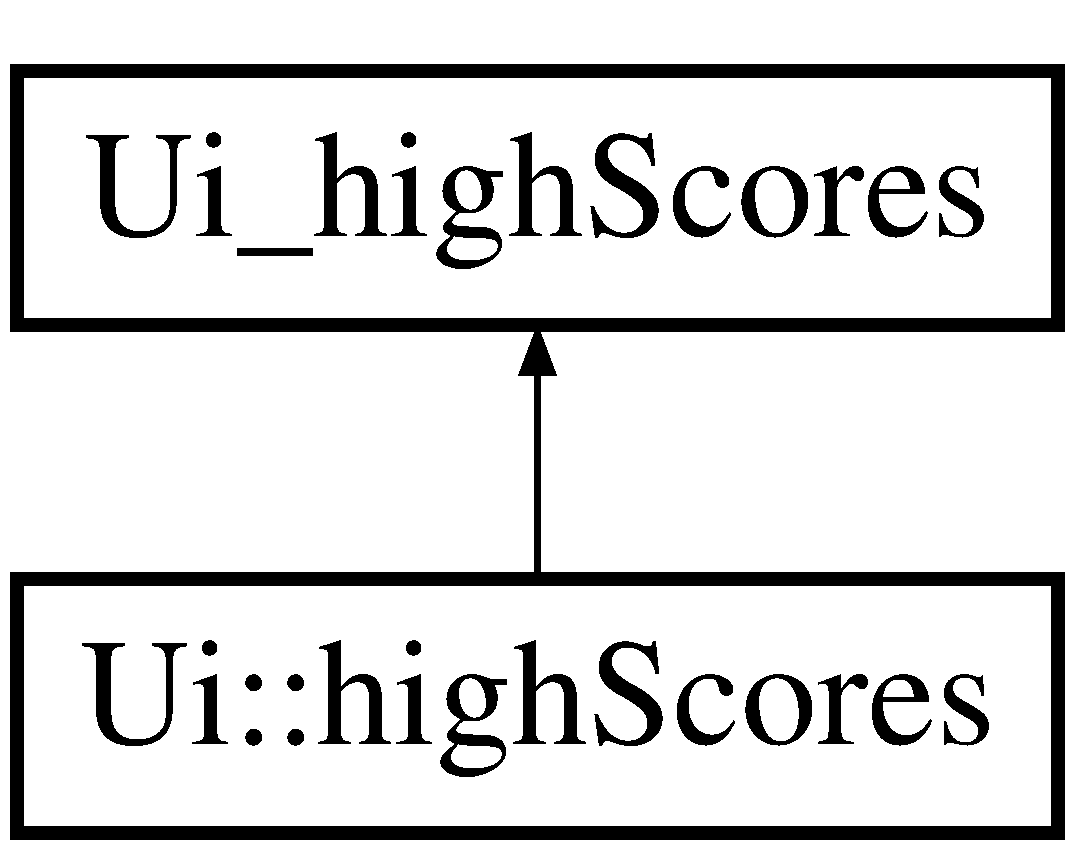
\includegraphics[height=2.000000cm]{classUi_1_1highScores}
\end{center}
\end{figure}
\subsection*{Additional Inherited Members}


The documentation for this class was generated from the following file\-:\begin{DoxyCompactItemize}
\item 
ui\-\_\-scoreboard.\-h\end{DoxyCompactItemize}

\hypertarget{classItemFactory}{\section{Item\-Factory Class Reference}
\label{classItemFactory}\index{Item\-Factory@{Item\-Factory}}
}
\subsection*{Static Public Member Functions}
\begin{DoxyCompactItemize}
\item 
\hypertarget{classItemFactory_a1efc7a13647cb8a221048900abcdc290}{static Q\-Graphics\-Item $\ast$ {\bfseries make} (\hyperlink{classConfigItem}{Config\-Item} $\ast$config)}\label{classItemFactory_a1efc7a13647cb8a221048900abcdc290}

\end{DoxyCompactItemize}


The documentation for this class was generated from the following files\-:\begin{DoxyCompactItemize}
\item 
itemfactory.\-h\item 
itemfactory.\-cpp\end{DoxyCompactItemize}

\hypertarget{classKeyEvent}{\section{Key\-Event Class Reference}
\label{classKeyEvent}\index{Key\-Event@{Key\-Event}}
}


Transport key stroke events.  




{\ttfamily \#include $<$Events.\-h$>$}

Inheritance diagram for Key\-Event\-:\begin{figure}[H]
\begin{center}
\leavevmode
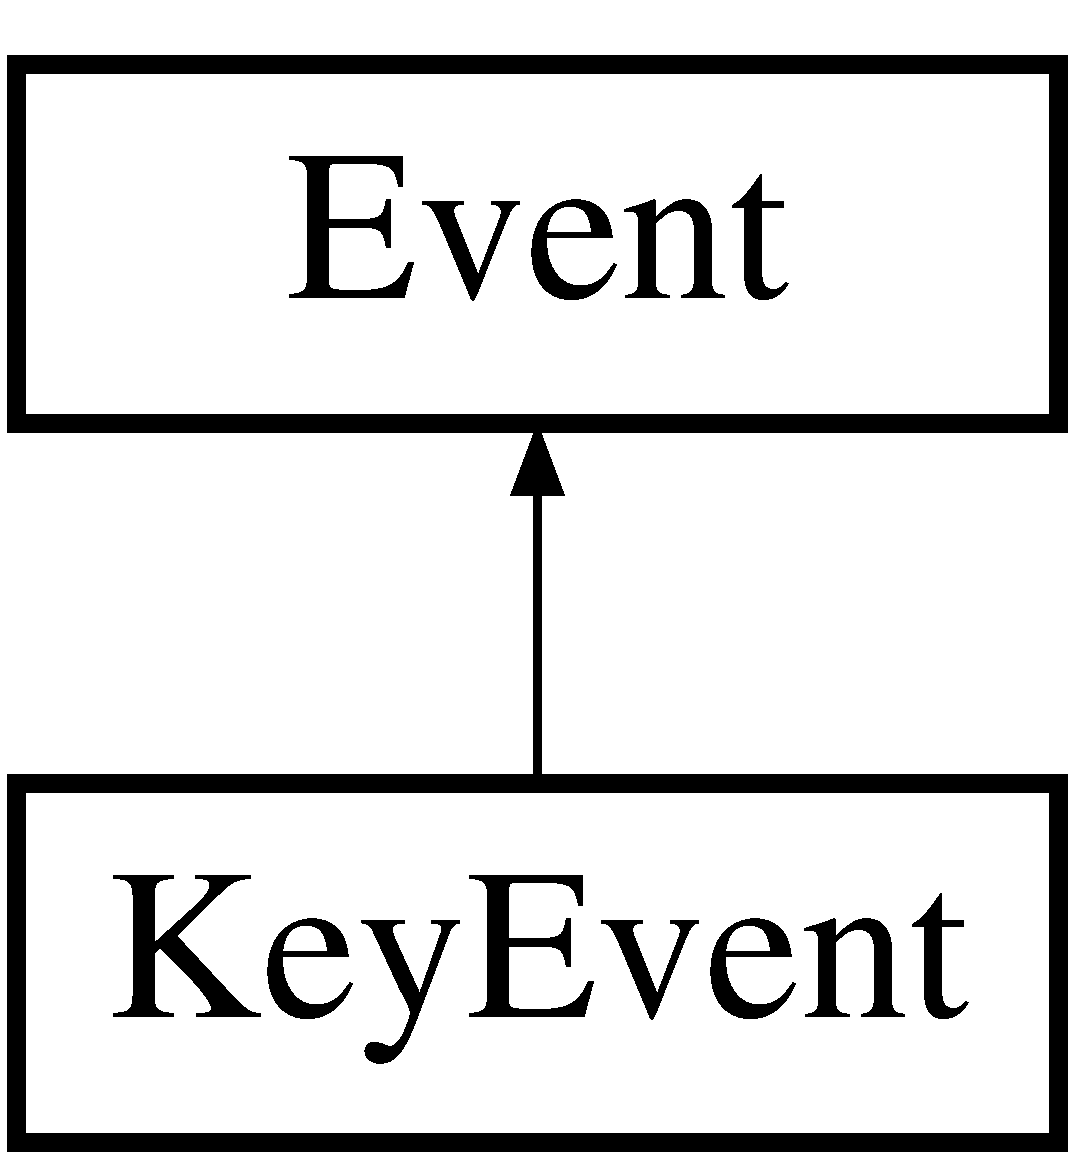
\includegraphics[height=2.000000cm]{classKeyEvent}
\end{center}
\end{figure}
\subsection*{Public Attributes}
\begin{DoxyCompactItemize}
\item 
int \hyperlink{classKeyEvent_a099e4f3c01870f67baffeba80b5c1860}{keycode}
\end{DoxyCompactItemize}
\subsection*{Additional Inherited Members}


\subsection{Detailed Description}
Transport key stroke events. 

\subsection{Member Data Documentation}
\hypertarget{classKeyEvent_a099e4f3c01870f67baffeba80b5c1860}{\index{Key\-Event@{Key\-Event}!keycode@{keycode}}
\index{keycode@{keycode}!KeyEvent@{Key\-Event}}
\subsubsection[{keycode}]{\setlength{\rightskip}{0pt plus 5cm}int Key\-Event\-::keycode}}\label{classKeyEvent_a099e4f3c01870f67baffeba80b5c1860}
Store the keycode to transport. 

The documentation for this class was generated from the following file\-:\begin{DoxyCompactItemize}
\item 
Events.\-h\end{DoxyCompactItemize}

\hypertarget{classLevel}{\section{Level Class Reference}
\label{classLevel}\index{Level@{Level}}
}


Implement levels and switching to next one.  




{\ttfamily \#include $<$level.\-h$>$}

Inheritance diagram for Level\-:\begin{figure}[H]
\begin{center}
\leavevmode
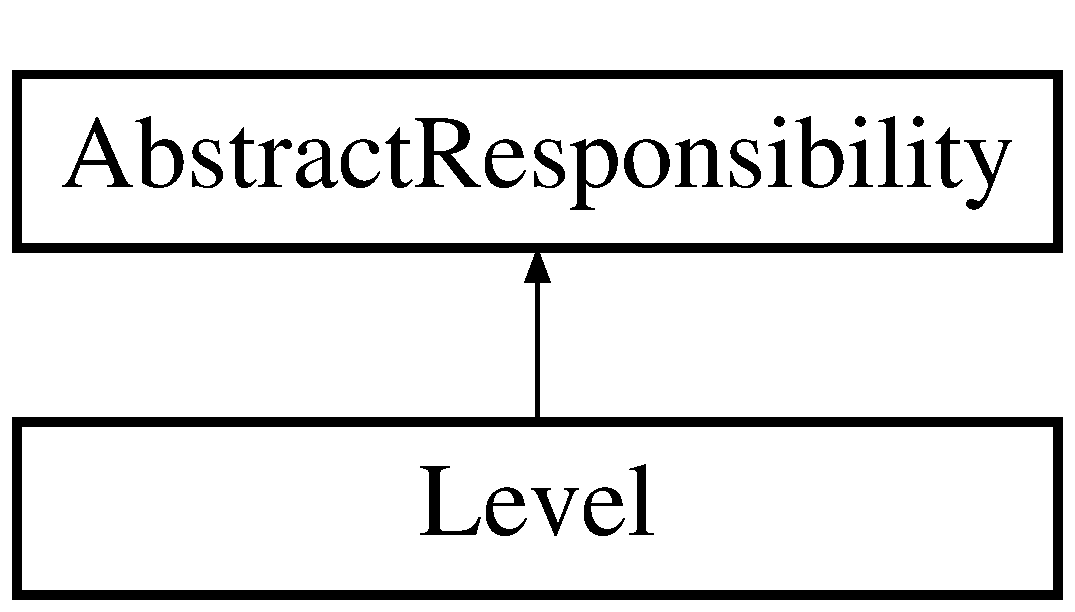
\includegraphics[height=2.000000cm]{classLevel}
\end{center}
\end{figure}
\subsection*{Public Member Functions}
\begin{DoxyCompactItemize}
\item 
\hyperlink{classLevel_a1ad0ac0368b30dd5389761c44e6b42db}{Level} (\hyperlink{classLevelConfigItem}{Level\-Config\-Item} const $\ast$)
\item 
\hyperlink{classLevel_a249eac1e8f19ff44134efa5e986feaca}{$\sim$\-Level} ()
\item 
void \hyperlink{classLevel_a01a06c7956b2090df3efb6c2834a8ee0}{handle\-Event} (\hyperlink{classEvent}{Event} $\ast$)
\item 
int \hyperlink{classLevel_ac06e7d9fa248ce159a4489b9db2e9a72}{get\-Level\-Num} () const 
\item 
int \hyperlink{classLevel_a321e86205d65be219d52200e62ffde55}{get\-Update\-Wait} () const 
\end{DoxyCompactItemize}
\subsection*{Additional Inherited Members}


\subsection{Detailed Description}
Implement levels and switching to next one. 

This class stores the information of the currently running level. It also stores a counter of how many blocks are present in the level and emits a level cleared event when all blocks are destroyed. 

\subsection{Constructor \& Destructor Documentation}
\hypertarget{classLevel_a1ad0ac0368b30dd5389761c44e6b42db}{\index{Level@{Level}!Level@{Level}}
\index{Level@{Level}!Level@{Level}}
\subsubsection[{Level}]{\setlength{\rightskip}{0pt plus 5cm}Level\-::\-Level (
\begin{DoxyParamCaption}
\item[{{\bf Level\-Config\-Item} const $\ast$}]{config}
\end{DoxyParamCaption}
)}}\label{classLevel_a1ad0ac0368b30dd5389761c44e6b42db}
Create the level from the config item. \hypertarget{classLevel_a249eac1e8f19ff44134efa5e986feaca}{\index{Level@{Level}!$\sim$\-Level@{$\sim$\-Level}}
\index{$\sim$\-Level@{$\sim$\-Level}!Level@{Level}}
\subsubsection[{$\sim$\-Level}]{\setlength{\rightskip}{0pt plus 5cm}Level\-::$\sim$\-Level (
\begin{DoxyParamCaption}
{}
\end{DoxyParamCaption}
)}}\label{classLevel_a249eac1e8f19ff44134efa5e986feaca}
Remove me from the chain of responsibilitiy. 

\subsection{Member Function Documentation}
\hypertarget{classLevel_ac06e7d9fa248ce159a4489b9db2e9a72}{\index{Level@{Level}!get\-Level\-Num@{get\-Level\-Num}}
\index{get\-Level\-Num@{get\-Level\-Num}!Level@{Level}}
\subsubsection[{get\-Level\-Num}]{\setlength{\rightskip}{0pt plus 5cm}int Level\-::get\-Level\-Num (
\begin{DoxyParamCaption}
{}
\end{DoxyParamCaption}
) const\hspace{0.3cm}{\ttfamily [inline]}}}\label{classLevel_ac06e7d9fa248ce159a4489b9db2e9a72}
Get the number of this level. \hypertarget{classLevel_a321e86205d65be219d52200e62ffde55}{\index{Level@{Level}!get\-Update\-Wait@{get\-Update\-Wait}}
\index{get\-Update\-Wait@{get\-Update\-Wait}!Level@{Level}}
\subsubsection[{get\-Update\-Wait}]{\setlength{\rightskip}{0pt plus 5cm}int Level\-::get\-Update\-Wait (
\begin{DoxyParamCaption}
{}
\end{DoxyParamCaption}
) const\hspace{0.3cm}{\ttfamily [inline]}}}\label{classLevel_a321e86205d65be219d52200e62ffde55}
Get the number of msec to wait between updates. \hypertarget{classLevel_a01a06c7956b2090df3efb6c2834a8ee0}{\index{Level@{Level}!handle\-Event@{handle\-Event}}
\index{handle\-Event@{handle\-Event}!Level@{Level}}
\subsubsection[{handle\-Event}]{\setlength{\rightskip}{0pt plus 5cm}void Level\-::handle\-Event (
\begin{DoxyParamCaption}
\item[{{\bf Event} $\ast$}]{ev}
\end{DoxyParamCaption}
)\hspace{0.3cm}{\ttfamily [virtual]}}}\label{classLevel_a01a06c7956b2090df3efb6c2834a8ee0}
Handle events of block deleted. 

Reimplemented from \hyperlink{classAbstractResponsibility_a14d885884ae4841dbe7c5824b986f2c9}{Abstract\-Responsibility}.



The documentation for this class was generated from the following files\-:\begin{DoxyCompactItemize}
\item 
level.\-h\item 
level.\-cpp\end{DoxyCompactItemize}

\hypertarget{classLevelClearedEvent}{\section{Level\-Cleared\-Event Class Reference}
\label{classLevelClearedEvent}\index{Level\-Cleared\-Event@{Level\-Cleared\-Event}}
}


Triggered when all blocks are removed from a scene.  




{\ttfamily \#include $<$Events.\-h$>$}

Inheritance diagram for Level\-Cleared\-Event\-:\begin{figure}[H]
\begin{center}
\leavevmode
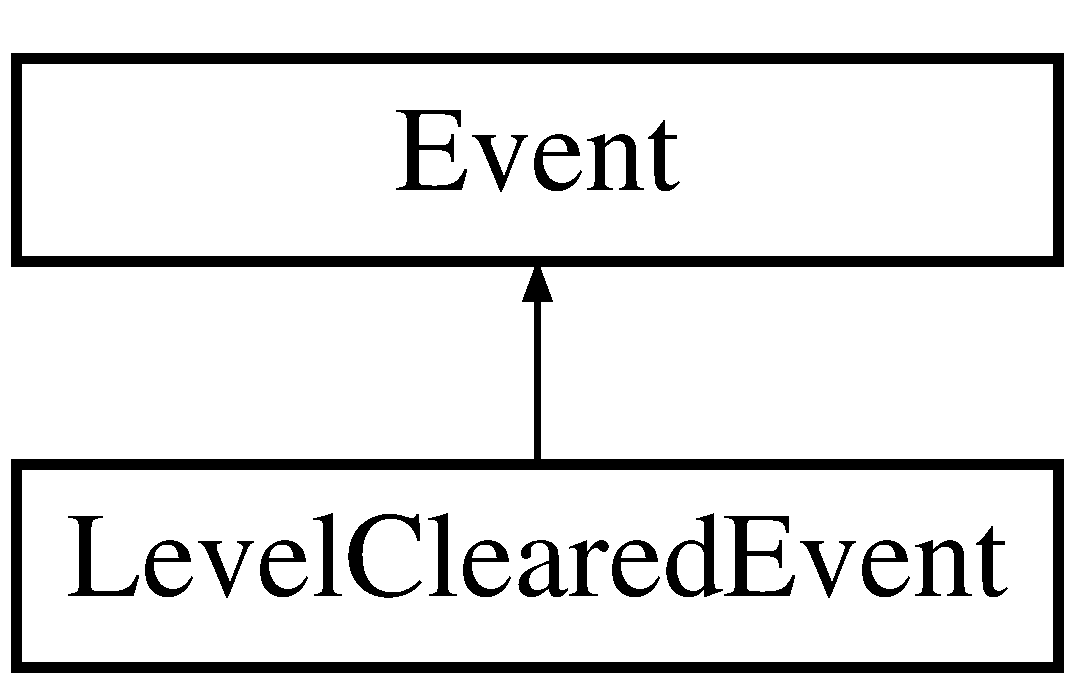
\includegraphics[height=2.000000cm]{classLevelClearedEvent}
\end{center}
\end{figure}
\subsection*{Additional Inherited Members}


\subsection{Detailed Description}
Triggered when all blocks are removed from a scene. 

The documentation for this class was generated from the following file\-:\begin{DoxyCompactItemize}
\item 
Events.\-h\end{DoxyCompactItemize}

\hypertarget{classLevelConfigItem}{\section{Level\-Config\-Item Class Reference}
\label{classLevelConfigItem}\index{Level\-Config\-Item@{Level\-Config\-Item}}
}


Store config-\/file data of a level.  




{\ttfamily \#include $<$levelconfigitem.\-h$>$}

Inheritance diagram for Level\-Config\-Item\-:\begin{figure}[H]
\begin{center}
\leavevmode
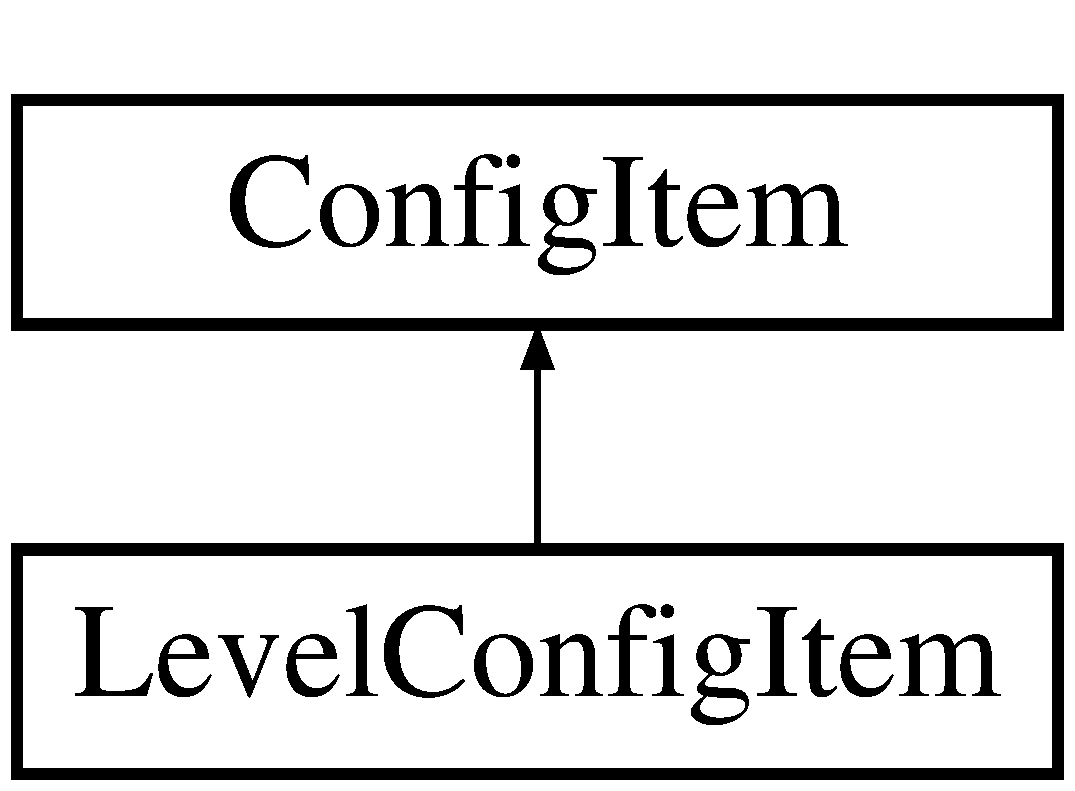
\includegraphics[height=2.000000cm]{classLevelConfigItem}
\end{center}
\end{figure}
\subsection*{Public Member Functions}
\begin{DoxyCompactItemize}
\item 
\hyperlink{classLevelConfigItem_abefbac4a4cf846ab666d8836472b91b6}{Level\-Config\-Item} ()
\item 
\hyperlink{classLevelConfigItem_ae75692250e03ea40d77853e5af1dd36d}{$\sim$\-Level\-Config\-Item} ()
\item 
bool \hyperlink{classLevelConfigItem_af717103b0881d4512dbee6f3c509c568}{validate} (int height, int width) const 
\item 
Item \hyperlink{classLevelConfigItem_aed6d6c4ff654506d582732a77ec96056}{get\-Item\-Type} () const 
\item 
void \hyperlink{classLevelConfigItem_a7a8b3d45729b0351ee590f7fdc5a4e5f}{add\-Parameter} (std\-::string name, double value)
\item 
\hyperlink{classConfigItem}{Config\-Item} $\ast$ \hyperlink{classLevelConfigItem_a4e47772ef1d7d5062979424129f4d3e4}{add} (\hyperlink{classConfigItem}{Config\-Item} $\ast$new\-Item)
\item 
void \hyperlink{classLevelConfigItem_aafa487a690ee7bea2111969dc4369ed2}{set\-Level\-Num} (int const n\-Level\-Num)
\item 
int \hyperlink{classLevelConfigItem_a828bcca5a829b7cb1df12b20406ae982}{get\-Level\-Num} () const 
\item 
void \hyperlink{classLevelConfigItem_ae49bc07589a7117d4aaecf4bf4c2376c}{set\-Update\-Delay} (const int n\-Update\-Wait)
\item 
int \hyperlink{classLevelConfigItem_a9e2c29bf67193b6ed6da6bd0c532cf80}{get\-Update\-Delay} () const 
\item 
\hyperlink{classConfigItem}{Config\-Item} $\ast$ \hyperlink{classLevelConfigItem_ab41db3f785b4210fb9a681379fdde0d9}{operator\mbox{[}$\,$\mbox{]}} (int i)
\item 
size\-\_\-t \hyperlink{classLevelConfigItem_a3b928feaf14e2e2e2e145ef0ffac566c}{size} () const 
\end{DoxyCompactItemize}


\subsection{Detailed Description}
Store config-\/file data of a level. 

Store the configuration file data of a level. Besides the configured blocks the number of the level is stored and the update intervall. A smaller update intervall make the ball faster, while leaving the paddle at the same reaction speed. \-:) 

\subsection{Constructor \& Destructor Documentation}
\hypertarget{classLevelConfigItem_abefbac4a4cf846ab666d8836472b91b6}{\index{Level\-Config\-Item@{Level\-Config\-Item}!Level\-Config\-Item@{Level\-Config\-Item}}
\index{Level\-Config\-Item@{Level\-Config\-Item}!LevelConfigItem@{Level\-Config\-Item}}
\subsubsection[{Level\-Config\-Item}]{\setlength{\rightskip}{0pt plus 5cm}Level\-Config\-Item\-::\-Level\-Config\-Item (
\begin{DoxyParamCaption}
{}
\end{DoxyParamCaption}
)}}\label{classLevelConfigItem_abefbac4a4cf846ab666d8836472b91b6}
Set default values. \hypertarget{classLevelConfigItem_ae75692250e03ea40d77853e5af1dd36d}{\index{Level\-Config\-Item@{Level\-Config\-Item}!$\sim$\-Level\-Config\-Item@{$\sim$\-Level\-Config\-Item}}
\index{$\sim$\-Level\-Config\-Item@{$\sim$\-Level\-Config\-Item}!LevelConfigItem@{Level\-Config\-Item}}
\subsubsection[{$\sim$\-Level\-Config\-Item}]{\setlength{\rightskip}{0pt plus 5cm}Level\-Config\-Item\-::$\sim$\-Level\-Config\-Item (
\begin{DoxyParamCaption}
{}
\end{DoxyParamCaption}
)}}\label{classLevelConfigItem_ae75692250e03ea40d77853e5af1dd36d}
On level destruction free the configured items. 

\subsection{Member Function Documentation}
\hypertarget{classLevelConfigItem_a4e47772ef1d7d5062979424129f4d3e4}{\index{Level\-Config\-Item@{Level\-Config\-Item}!add@{add}}
\index{add@{add}!LevelConfigItem@{Level\-Config\-Item}}
\subsubsection[{add}]{\setlength{\rightskip}{0pt plus 5cm}{\bf Config\-Item} $\ast$ Level\-Config\-Item\-::add (
\begin{DoxyParamCaption}
\item[{{\bf Config\-Item} $\ast$}]{new\-Item}
\end{DoxyParamCaption}
)}}\label{classLevelConfigItem_a4e47772ef1d7d5062979424129f4d3e4}
Add a config item to this levels set. \hypertarget{classLevelConfigItem_a7a8b3d45729b0351ee590f7fdc5a4e5f}{\index{Level\-Config\-Item@{Level\-Config\-Item}!add\-Parameter@{add\-Parameter}}
\index{add\-Parameter@{add\-Parameter}!LevelConfigItem@{Level\-Config\-Item}}
\subsubsection[{add\-Parameter}]{\setlength{\rightskip}{0pt plus 5cm}void Level\-Config\-Item\-::add\-Parameter (
\begin{DoxyParamCaption}
\item[{std\-::string}]{name, }
\item[{double}]{value}
\end{DoxyParamCaption}
)\hspace{0.3cm}{\ttfamily [virtual]}}}\label{classLevelConfigItem_a7a8b3d45729b0351ee590f7fdc5a4e5f}
Add parameters known to the level. 

Implements \hyperlink{classConfigItem}{Config\-Item}.

\hypertarget{classLevelConfigItem_aed6d6c4ff654506d582732a77ec96056}{\index{Level\-Config\-Item@{Level\-Config\-Item}!get\-Item\-Type@{get\-Item\-Type}}
\index{get\-Item\-Type@{get\-Item\-Type}!LevelConfigItem@{Level\-Config\-Item}}
\subsubsection[{get\-Item\-Type}]{\setlength{\rightskip}{0pt plus 5cm}Item Level\-Config\-Item\-::get\-Item\-Type (
\begin{DoxyParamCaption}
{}
\end{DoxyParamCaption}
) const\hspace{0.3cm}{\ttfamily [virtual]}}}\label{classLevelConfigItem_aed6d6c4ff654506d582732a77ec96056}
Set this items type to \hyperlink{classLevel}{Level}. 

Implements \hyperlink{classConfigItem}{Config\-Item}.

\hypertarget{classLevelConfigItem_a828bcca5a829b7cb1df12b20406ae982}{\index{Level\-Config\-Item@{Level\-Config\-Item}!get\-Level\-Num@{get\-Level\-Num}}
\index{get\-Level\-Num@{get\-Level\-Num}!LevelConfigItem@{Level\-Config\-Item}}
\subsubsection[{get\-Level\-Num}]{\setlength{\rightskip}{0pt plus 5cm}int Level\-Config\-Item\-::get\-Level\-Num (
\begin{DoxyParamCaption}
{}
\end{DoxyParamCaption}
) const\hspace{0.3cm}{\ttfamily [inline]}}}\label{classLevelConfigItem_a828bcca5a829b7cb1df12b20406ae982}
Get the number of this level. \hypertarget{classLevelConfigItem_a9e2c29bf67193b6ed6da6bd0c532cf80}{\index{Level\-Config\-Item@{Level\-Config\-Item}!get\-Update\-Delay@{get\-Update\-Delay}}
\index{get\-Update\-Delay@{get\-Update\-Delay}!LevelConfigItem@{Level\-Config\-Item}}
\subsubsection[{get\-Update\-Delay}]{\setlength{\rightskip}{0pt plus 5cm}int Level\-Config\-Item\-::get\-Update\-Delay (
\begin{DoxyParamCaption}
{}
\end{DoxyParamCaption}
) const\hspace{0.3cm}{\ttfamily [inline]}}}\label{classLevelConfigItem_a9e2c29bf67193b6ed6da6bd0c532cf80}
Get the update delay for this level. \hypertarget{classLevelConfigItem_ab41db3f785b4210fb9a681379fdde0d9}{\index{Level\-Config\-Item@{Level\-Config\-Item}!operator\mbox{[}$\,$\mbox{]}@{operator[]}}
\index{operator\mbox{[}$\,$\mbox{]}@{operator[]}!LevelConfigItem@{Level\-Config\-Item}}
\subsubsection[{operator[]}]{\setlength{\rightskip}{0pt plus 5cm}{\bf Config\-Item}$\ast$ Level\-Config\-Item\-::operator\mbox{[}$\,$\mbox{]} (
\begin{DoxyParamCaption}
\item[{int}]{i}
\end{DoxyParamCaption}
)\hspace{0.3cm}{\ttfamily [inline]}}}\label{classLevelConfigItem_ab41db3f785b4210fb9a681379fdde0d9}
Get the i-\/th item. \hypertarget{classLevelConfigItem_aafa487a690ee7bea2111969dc4369ed2}{\index{Level\-Config\-Item@{Level\-Config\-Item}!set\-Level\-Num@{set\-Level\-Num}}
\index{set\-Level\-Num@{set\-Level\-Num}!LevelConfigItem@{Level\-Config\-Item}}
\subsubsection[{set\-Level\-Num}]{\setlength{\rightskip}{0pt plus 5cm}void Level\-Config\-Item\-::set\-Level\-Num (
\begin{DoxyParamCaption}
\item[{int const}]{n\-Level\-Num}
\end{DoxyParamCaption}
)\hspace{0.3cm}{\ttfamily [inline]}}}\label{classLevelConfigItem_aafa487a690ee7bea2111969dc4369ed2}
Set the number of this level. \hypertarget{classLevelConfigItem_ae49bc07589a7117d4aaecf4bf4c2376c}{\index{Level\-Config\-Item@{Level\-Config\-Item}!set\-Update\-Delay@{set\-Update\-Delay}}
\index{set\-Update\-Delay@{set\-Update\-Delay}!LevelConfigItem@{Level\-Config\-Item}}
\subsubsection[{set\-Update\-Delay}]{\setlength{\rightskip}{0pt plus 5cm}void Level\-Config\-Item\-::set\-Update\-Delay (
\begin{DoxyParamCaption}
\item[{const int}]{n\-Update\-Wait}
\end{DoxyParamCaption}
)\hspace{0.3cm}{\ttfamily [inline]}}}\label{classLevelConfigItem_ae49bc07589a7117d4aaecf4bf4c2376c}
Set the update delay for this level. \hypertarget{classLevelConfigItem_a3b928feaf14e2e2e2e145ef0ffac566c}{\index{Level\-Config\-Item@{Level\-Config\-Item}!size@{size}}
\index{size@{size}!LevelConfigItem@{Level\-Config\-Item}}
\subsubsection[{size}]{\setlength{\rightskip}{0pt plus 5cm}size\-\_\-t Level\-Config\-Item\-::size (
\begin{DoxyParamCaption}
{}
\end{DoxyParamCaption}
) const\hspace{0.3cm}{\ttfamily [inline]}}}\label{classLevelConfigItem_a3b928feaf14e2e2e2e145ef0ffac566c}
Return the number of elements in this level. \hypertarget{classLevelConfigItem_af717103b0881d4512dbee6f3c509c568}{\index{Level\-Config\-Item@{Level\-Config\-Item}!validate@{validate}}
\index{validate@{validate}!LevelConfigItem@{Level\-Config\-Item}}
\subsubsection[{validate}]{\setlength{\rightskip}{0pt plus 5cm}bool Level\-Config\-Item\-::validate (
\begin{DoxyParamCaption}
\item[{int}]{height, }
\item[{int}]{width}
\end{DoxyParamCaption}
) const\hspace{0.3cm}{\ttfamily [virtual]}}}\label{classLevelConfigItem_af717103b0881d4512dbee6f3c509c568}
Validate that this collection of configured items is in the scene. 

Implements \hyperlink{classConfigItem_a0ffeae3ab9688202ad167e15ccb3be6d}{Config\-Item}.



The documentation for this class was generated from the following files\-:\begin{DoxyCompactItemize}
\item 
levelconfigitem.\-h\item 
levelconfigitem.\-cpp\end{DoxyCompactItemize}

\hypertarget{classOutOfLivesEvent}{\section{Out\-Of\-Lives\-Event Class Reference}
\label{classOutOfLivesEvent}\index{Out\-Of\-Lives\-Event@{Out\-Of\-Lives\-Event}}
}


Triggered when the lives reaches zero.  




{\ttfamily \#include $<$Events.\-h$>$}

Inheritance diagram for Out\-Of\-Lives\-Event\-:\begin{figure}[H]
\begin{center}
\leavevmode
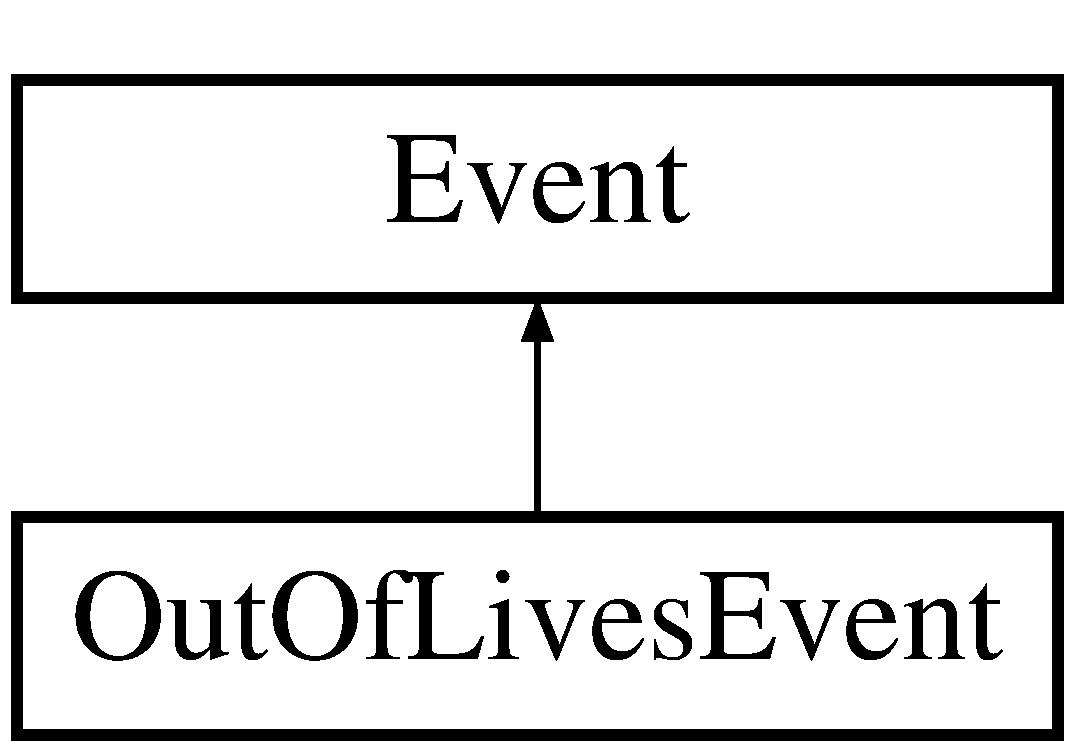
\includegraphics[height=2.000000cm]{classOutOfLivesEvent}
\end{center}
\end{figure}
\subsection*{Additional Inherited Members}


\subsection{Detailed Description}
Triggered when the lives reaches zero. 

The documentation for this class was generated from the following file\-:\begin{DoxyCompactItemize}
\item 
Events.\-h\end{DoxyCompactItemize}

\hypertarget{classPaddle}{\section{Paddle Class Reference}
\label{classPaddle}\index{Paddle@{Paddle}}
}


Implement the paddle a the bottom of the screen.  




{\ttfamily \#include $<$paddle.\-h$>$}

Inheritance diagram for Paddle\-:\begin{figure}[H]
\begin{center}
\leavevmode
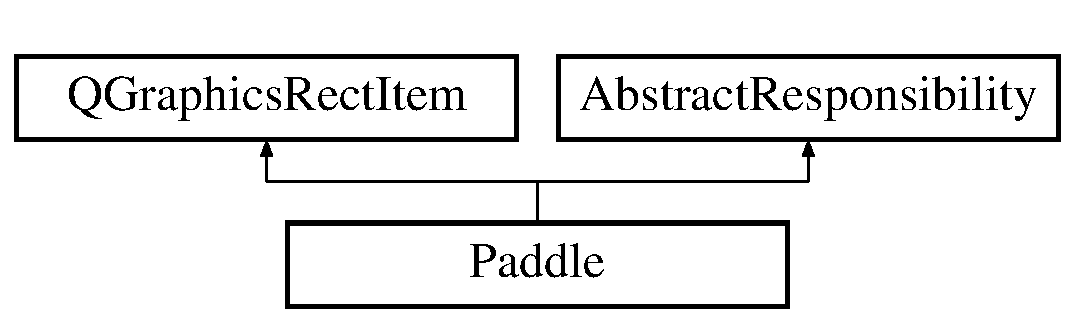
\includegraphics[height=2.000000cm]{classPaddle}
\end{center}
\end{figure}
\subsection*{Public Member Functions}
\begin{DoxyCompactItemize}
\item 
\hyperlink{classPaddle_ad796bdd2f07b024b1c518439149a2866}{Paddle} (\hyperlink{classPaddleConfigItem}{Paddle\-Config\-Item} $\ast$)
\item 
void \hyperlink{classPaddle_aef40328563790e25a73ee4c6b58fa390}{handle\-Event} (\hyperlink{classEvent}{Event} $\ast$event)
\end{DoxyCompactItemize}
\subsection*{Protected Member Functions}
\begin{DoxyCompactItemize}
\item 
Q\-Variant \hyperlink{classPaddle_ad2fa885cc0f5fdabb53429b19569a997}{item\-Change} (Graphics\-Item\-Change change, const Q\-Variant \&value)
\end{DoxyCompactItemize}
\subsection*{Additional Inherited Members}


\subsection{Detailed Description}
Implement the paddle a the bottom of the screen. 

The paddle is used to let the ball bounce of. Furthermore does it store the number of its lives and is also responsible for displaying them. The paddle observes the chain of responsibility to look for Ball\-Lost\-Events, certain key stroke events and may trigger the Out\-Of\-Lives event, when all lives are void. When a Out\-Of\-Lives event is seen, but lives are still present, then the game ends because all blocks have been destroyed and no more levels are present. The paddle then adds 100 points for every live left. 

\subsection{Constructor \& Destructor Documentation}
\hypertarget{classPaddle_ad796bdd2f07b024b1c518439149a2866}{\index{Paddle@{Paddle}!Paddle@{Paddle}}
\index{Paddle@{Paddle}!Paddle@{Paddle}}
\subsubsection[{Paddle}]{\setlength{\rightskip}{0pt plus 5cm}Paddle\-::\-Paddle (
\begin{DoxyParamCaption}
\item[{{\bf Paddle\-Config\-Item} $\ast$}]{config}
\end{DoxyParamCaption}
)}}\label{classPaddle_ad796bdd2f07b024b1c518439149a2866}
Create a new paddle to let the ball bounce of. 

\subsection{Member Function Documentation}
\hypertarget{classPaddle_aef40328563790e25a73ee4c6b58fa390}{\index{Paddle@{Paddle}!handle\-Event@{handle\-Event}}
\index{handle\-Event@{handle\-Event}!Paddle@{Paddle}}
\subsubsection[{handle\-Event}]{\setlength{\rightskip}{0pt plus 5cm}void Paddle\-::handle\-Event (
\begin{DoxyParamCaption}
\item[{{\bf Event} $\ast$}]{event}
\end{DoxyParamCaption}
)\hspace{0.3cm}{\ttfamily [virtual]}}}\label{classPaddle_aef40328563790e25a73ee4c6b58fa390}
Implement handling of K and L keys here. K moves the paddle left and L right. 

Reimplemented from \hyperlink{classAbstractResponsibility_a14d885884ae4841dbe7c5824b986f2c9}{Abstract\-Responsibility}.

\hypertarget{classPaddle_ad2fa885cc0f5fdabb53429b19569a997}{\index{Paddle@{Paddle}!item\-Change@{item\-Change}}
\index{item\-Change@{item\-Change}!Paddle@{Paddle}}
\subsubsection[{item\-Change}]{\setlength{\rightskip}{0pt plus 5cm}Q\-Variant Paddle\-::item\-Change (
\begin{DoxyParamCaption}
\item[{Graphics\-Item\-Change}]{change, }
\item[{const Q\-Variant \&}]{value}
\end{DoxyParamCaption}
)\hspace{0.3cm}{\ttfamily [protected]}}}\label{classPaddle_ad2fa885cc0f5fdabb53429b19569a997}
When the item is added to the scene then a Item\-Scene\-Changed notify is send. On such an event add the lives\-Display to the scene.

When the item is added to the scene then a Item\-Scene\-Changed notify is send. 

The documentation for this class was generated from the following files\-:\begin{DoxyCompactItemize}
\item 
paddle.\-h\item 
paddle.\-cpp\end{DoxyCompactItemize}

\hypertarget{classPaddleConfigItem}{\section{Paddle\-Config\-Item Class Reference}
\label{classPaddleConfigItem}\index{Paddle\-Config\-Item@{Paddle\-Config\-Item}}
}


Store and propagate the paddle's configuration.  




{\ttfamily \#include $<$paddleconfigitem.\-h$>$}

Inheritance diagram for Paddle\-Config\-Item\-:\begin{figure}[H]
\begin{center}
\leavevmode
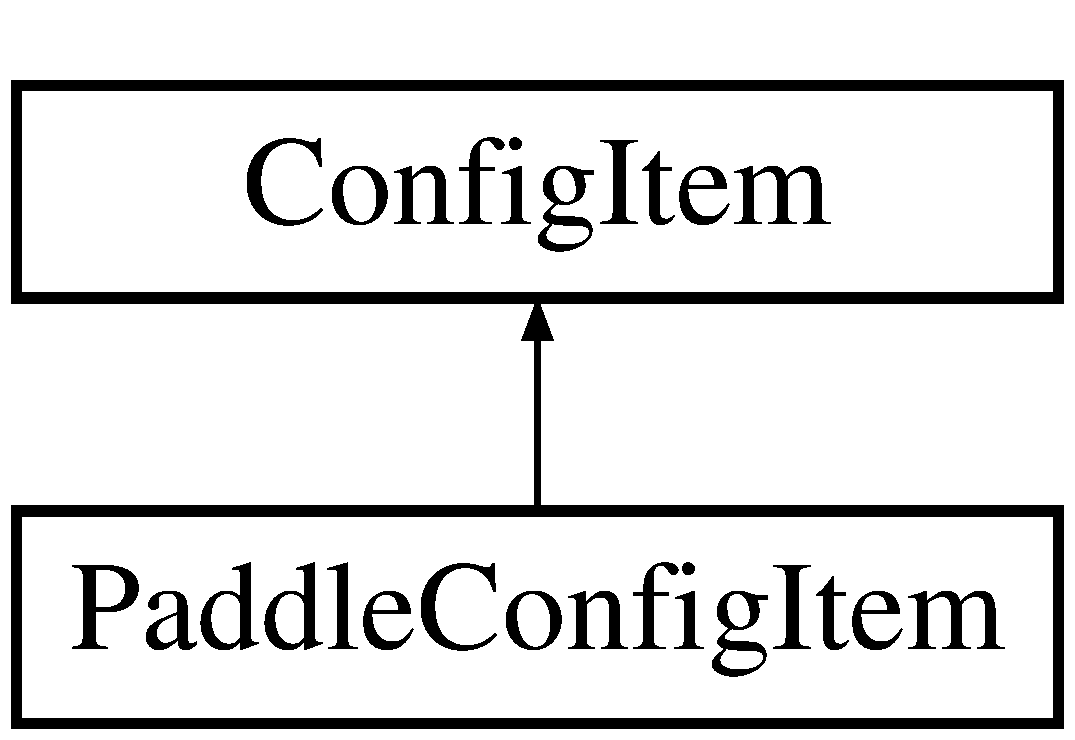
\includegraphics[height=2.000000cm]{classPaddleConfigItem}
\end{center}
\end{figure}
\subsection*{Public Member Functions}
\begin{DoxyCompactItemize}
\item 
\hyperlink{classPaddleConfigItem_aaf8327c16b6ea75fcc4472635d8d203a}{Paddle\-Config\-Item} ()
\item 
bool \hyperlink{classPaddleConfigItem_a4471662990213dab829792a73683fd0f}{validate} (int height, int width) const 
\item 
Item \hyperlink{classPaddleConfigItem_a9aff3ad1cce28b13cfb1262ce6d73acc}{get\-Item\-Type} () const 
\item 
Q\-Rect const \hyperlink{classPaddleConfigItem_ac4fb268e37165db4eb1367f69cdb7bc7}{get\-Rect} () const 
\item 
Q\-Point const \hyperlink{classPaddleConfigItem_ab089e52a94ef9ec97b2237546254ef54}{get\-Pos} () const 
\item 
void \hyperlink{classPaddleConfigItem_ad7b5b50b1e480e1f0b2b653e05944297}{add\-Parameter} (std\-::string name, double value)
\item 
int \hyperlink{classPaddleConfigItem_a69c5d3519bcaac03472d0a4377c0f45f}{get\-X\-Coordinate} () const 
\item 
void \hyperlink{classPaddleConfigItem_aeef3371c9228bd742a44d01bf54bb99c}{set\-X\-Coordinate} (int)
\item 
int \hyperlink{classPaddleConfigItem_a9750f9729e7a200de27b988407791b16}{get\-Y\-Coordinate} () const 
\item 
void \hyperlink{classPaddleConfigItem_ad6247bbad6123b0f294bbc49c9d82bd3}{set\-Y\-Coordinate} (int)
\item 
float \hyperlink{classPaddleConfigItem_ae91bd3249691e453cb70b5cd105c3254}{get\-Width} () const 
\item 
void \hyperlink{classPaddleConfigItem_a1ed5776eb3a49f8f6f0a7db8cd75d24b}{set\-Width} (float)
\item 
float \hyperlink{classPaddleConfigItem_a543c31554ea6fd4230ce741f7896c655}{get\-Height} () const 
\item 
void \hyperlink{classPaddleConfigItem_a36d85ab3cbe8bf6ad7fa1aa4be04bf67}{set\-Height} (float)
\item 
Q\-Color \hyperlink{classPaddleConfigItem_a3fb77c280dbed567ae5f6dd5e5b875ca}{get\-Color} () const 
\item 
void \hyperlink{classPaddleConfigItem_a2fc99562dc100b5a8a5b2f6aad8ec3a2}{set\-Hue} (float)
\item 
unsigned int \hyperlink{classPaddleConfigItem_a425e6121ec4927ee5c3979a5a8d44c53}{get\-Lives} () const 
\item 
void \hyperlink{classPaddleConfigItem_a20233cf30a4363ce3fcfd65d157ed84a}{set\-Lives} (unsigned int lives)
\end{DoxyCompactItemize}


\subsection{Detailed Description}
Store and propagate the paddle's configuration. 

Store the configuration options for a paddle. This class essentially is a copy from the \hyperlink{classBlockConfigItem}{Block\-Config\-Item} with some internal changes. 

\subsection{Constructor \& Destructor Documentation}
\hypertarget{classPaddleConfigItem_aaf8327c16b6ea75fcc4472635d8d203a}{\index{Paddle\-Config\-Item@{Paddle\-Config\-Item}!Paddle\-Config\-Item@{Paddle\-Config\-Item}}
\index{Paddle\-Config\-Item@{Paddle\-Config\-Item}!PaddleConfigItem@{Paddle\-Config\-Item}}
\subsubsection[{Paddle\-Config\-Item}]{\setlength{\rightskip}{0pt plus 5cm}Paddle\-Config\-Item\-::\-Paddle\-Config\-Item (
\begin{DoxyParamCaption}
{}
\end{DoxyParamCaption}
)}}\label{classPaddleConfigItem_aaf8327c16b6ea75fcc4472635d8d203a}
Set defaults for attributes. 

\subsection{Member Function Documentation}
\hypertarget{classPaddleConfigItem_ad7b5b50b1e480e1f0b2b653e05944297}{\index{Paddle\-Config\-Item@{Paddle\-Config\-Item}!add\-Parameter@{add\-Parameter}}
\index{add\-Parameter@{add\-Parameter}!PaddleConfigItem@{Paddle\-Config\-Item}}
\subsubsection[{add\-Parameter}]{\setlength{\rightskip}{0pt plus 5cm}void Paddle\-Config\-Item\-::add\-Parameter (
\begin{DoxyParamCaption}
\item[{std\-::string}]{name, }
\item[{double}]{value}
\end{DoxyParamCaption}
)\hspace{0.3cm}{\ttfamily [virtual]}}}\label{classPaddleConfigItem_ad7b5b50b1e480e1f0b2b653e05944297}
In the configuration file after a P\-A\-D\-D\-L\-E section a parameter was found. Check if it is suitable for the paddle. 

Implements \hyperlink{classConfigItem}{Config\-Item}.

\hypertarget{classPaddleConfigItem_a3fb77c280dbed567ae5f6dd5e5b875ca}{\index{Paddle\-Config\-Item@{Paddle\-Config\-Item}!get\-Color@{get\-Color}}
\index{get\-Color@{get\-Color}!PaddleConfigItem@{Paddle\-Config\-Item}}
\subsubsection[{get\-Color}]{\setlength{\rightskip}{0pt plus 5cm}Q\-Color Paddle\-Config\-Item\-::get\-Color (
\begin{DoxyParamCaption}
{}
\end{DoxyParamCaption}
) const}}\label{classPaddleConfigItem_a3fb77c280dbed567ae5f6dd5e5b875ca}
Get the color of the paddle. \hypertarget{classPaddleConfigItem_a543c31554ea6fd4230ce741f7896c655}{\index{Paddle\-Config\-Item@{Paddle\-Config\-Item}!get\-Height@{get\-Height}}
\index{get\-Height@{get\-Height}!PaddleConfigItem@{Paddle\-Config\-Item}}
\subsubsection[{get\-Height}]{\setlength{\rightskip}{0pt plus 5cm}float Paddle\-Config\-Item\-::get\-Height (
\begin{DoxyParamCaption}
{}
\end{DoxyParamCaption}
) const}}\label{classPaddleConfigItem_a543c31554ea6fd4230ce741f7896c655}
Get the height of the paddle. \hypertarget{classPaddleConfigItem_a9aff3ad1cce28b13cfb1262ce6d73acc}{\index{Paddle\-Config\-Item@{Paddle\-Config\-Item}!get\-Item\-Type@{get\-Item\-Type}}
\index{get\-Item\-Type@{get\-Item\-Type}!PaddleConfigItem@{Paddle\-Config\-Item}}
\subsubsection[{get\-Item\-Type}]{\setlength{\rightskip}{0pt plus 5cm}Item Paddle\-Config\-Item\-::get\-Item\-Type (
\begin{DoxyParamCaption}
{}
\end{DoxyParamCaption}
) const\hspace{0.3cm}{\ttfamily [virtual]}}}\label{classPaddleConfigItem_a9aff3ad1cce28b13cfb1262ce6d73acc}
Identify us as a paddle. 

Implements \hyperlink{classConfigItem}{Config\-Item}.

\hypertarget{classPaddleConfigItem_a425e6121ec4927ee5c3979a5a8d44c53}{\index{Paddle\-Config\-Item@{Paddle\-Config\-Item}!get\-Lives@{get\-Lives}}
\index{get\-Lives@{get\-Lives}!PaddleConfigItem@{Paddle\-Config\-Item}}
\subsubsection[{get\-Lives}]{\setlength{\rightskip}{0pt plus 5cm}unsigned int Paddle\-Config\-Item\-::get\-Lives (
\begin{DoxyParamCaption}
{}
\end{DoxyParamCaption}
) const}}\label{classPaddleConfigItem_a425e6121ec4927ee5c3979a5a8d44c53}
Get the initial number of lives of this paddle.

Get and set the initial number of lives of this paddle. \hypertarget{classPaddleConfigItem_ab089e52a94ef9ec97b2237546254ef54}{\index{Paddle\-Config\-Item@{Paddle\-Config\-Item}!get\-Pos@{get\-Pos}}
\index{get\-Pos@{get\-Pos}!PaddleConfigItem@{Paddle\-Config\-Item}}
\subsubsection[{get\-Pos}]{\setlength{\rightskip}{0pt plus 5cm}Q\-Point const Paddle\-Config\-Item\-::get\-Pos (
\begin{DoxyParamCaption}
{}
\end{DoxyParamCaption}
) const\hspace{0.3cm}{\ttfamily [inline]}}}\label{classPaddleConfigItem_ab089e52a94ef9ec97b2237546254ef54}
Give the initial position of this paddle. \hypertarget{classPaddleConfigItem_ac4fb268e37165db4eb1367f69cdb7bc7}{\index{Paddle\-Config\-Item@{Paddle\-Config\-Item}!get\-Rect@{get\-Rect}}
\index{get\-Rect@{get\-Rect}!PaddleConfigItem@{Paddle\-Config\-Item}}
\subsubsection[{get\-Rect}]{\setlength{\rightskip}{0pt plus 5cm}Q\-Rect const Paddle\-Config\-Item\-::get\-Rect (
\begin{DoxyParamCaption}
{}
\end{DoxyParamCaption}
) const\hspace{0.3cm}{\ttfamily [inline]}}}\label{classPaddleConfigItem_ac4fb268e37165db4eb1367f69cdb7bc7}
For easy creation of a graphics item, create a rect here. \hypertarget{classPaddleConfigItem_ae91bd3249691e453cb70b5cd105c3254}{\index{Paddle\-Config\-Item@{Paddle\-Config\-Item}!get\-Width@{get\-Width}}
\index{get\-Width@{get\-Width}!PaddleConfigItem@{Paddle\-Config\-Item}}
\subsubsection[{get\-Width}]{\setlength{\rightskip}{0pt plus 5cm}float Paddle\-Config\-Item\-::get\-Width (
\begin{DoxyParamCaption}
{}
\end{DoxyParamCaption}
) const}}\label{classPaddleConfigItem_ae91bd3249691e453cb70b5cd105c3254}
Get the width of the paddle. \hypertarget{classPaddleConfigItem_a69c5d3519bcaac03472d0a4377c0f45f}{\index{Paddle\-Config\-Item@{Paddle\-Config\-Item}!get\-X\-Coordinate@{get\-X\-Coordinate}}
\index{get\-X\-Coordinate@{get\-X\-Coordinate}!PaddleConfigItem@{Paddle\-Config\-Item}}
\subsubsection[{get\-X\-Coordinate}]{\setlength{\rightskip}{0pt plus 5cm}int Paddle\-Config\-Item\-::get\-X\-Coordinate (
\begin{DoxyParamCaption}
{}
\end{DoxyParamCaption}
) const}}\label{classPaddleConfigItem_a69c5d3519bcaac03472d0a4377c0f45f}
Get the x coordinate. \hypertarget{classPaddleConfigItem_a9750f9729e7a200de27b988407791b16}{\index{Paddle\-Config\-Item@{Paddle\-Config\-Item}!get\-Y\-Coordinate@{get\-Y\-Coordinate}}
\index{get\-Y\-Coordinate@{get\-Y\-Coordinate}!PaddleConfigItem@{Paddle\-Config\-Item}}
\subsubsection[{get\-Y\-Coordinate}]{\setlength{\rightskip}{0pt plus 5cm}int Paddle\-Config\-Item\-::get\-Y\-Coordinate (
\begin{DoxyParamCaption}
{}
\end{DoxyParamCaption}
) const}}\label{classPaddleConfigItem_a9750f9729e7a200de27b988407791b16}
Get the y coordinate. \hypertarget{classPaddleConfigItem_a36d85ab3cbe8bf6ad7fa1aa4be04bf67}{\index{Paddle\-Config\-Item@{Paddle\-Config\-Item}!set\-Height@{set\-Height}}
\index{set\-Height@{set\-Height}!PaddleConfigItem@{Paddle\-Config\-Item}}
\subsubsection[{set\-Height}]{\setlength{\rightskip}{0pt plus 5cm}void Paddle\-Config\-Item\-::set\-Height (
\begin{DoxyParamCaption}
\item[{float}]{height}
\end{DoxyParamCaption}
)}}\label{classPaddleConfigItem_a36d85ab3cbe8bf6ad7fa1aa4be04bf67}
Set the height of the paddle. \hypertarget{classPaddleConfigItem_a2fc99562dc100b5a8a5b2f6aad8ec3a2}{\index{Paddle\-Config\-Item@{Paddle\-Config\-Item}!set\-Hue@{set\-Hue}}
\index{set\-Hue@{set\-Hue}!PaddleConfigItem@{Paddle\-Config\-Item}}
\subsubsection[{set\-Hue}]{\setlength{\rightskip}{0pt plus 5cm}void Paddle\-Config\-Item\-::set\-Hue (
\begin{DoxyParamCaption}
\item[{float}]{color\-Hue}
\end{DoxyParamCaption}
)}}\label{classPaddleConfigItem_a2fc99562dc100b5a8a5b2f6aad8ec3a2}
Set the color hue of the paddle. \hypertarget{classPaddleConfigItem_a20233cf30a4363ce3fcfd65d157ed84a}{\index{Paddle\-Config\-Item@{Paddle\-Config\-Item}!set\-Lives@{set\-Lives}}
\index{set\-Lives@{set\-Lives}!PaddleConfigItem@{Paddle\-Config\-Item}}
\subsubsection[{set\-Lives}]{\setlength{\rightskip}{0pt plus 5cm}void Paddle\-Config\-Item\-::set\-Lives (
\begin{DoxyParamCaption}
\item[{unsigned int}]{lives}
\end{DoxyParamCaption}
)}}\label{classPaddleConfigItem_a20233cf30a4363ce3fcfd65d157ed84a}
Set the initial number of lives of this paddle. \hypertarget{classPaddleConfigItem_a1ed5776eb3a49f8f6f0a7db8cd75d24b}{\index{Paddle\-Config\-Item@{Paddle\-Config\-Item}!set\-Width@{set\-Width}}
\index{set\-Width@{set\-Width}!PaddleConfigItem@{Paddle\-Config\-Item}}
\subsubsection[{set\-Width}]{\setlength{\rightskip}{0pt plus 5cm}void Paddle\-Config\-Item\-::set\-Width (
\begin{DoxyParamCaption}
\item[{float}]{width}
\end{DoxyParamCaption}
)}}\label{classPaddleConfigItem_a1ed5776eb3a49f8f6f0a7db8cd75d24b}
Set the width of the paddle. \hypertarget{classPaddleConfigItem_aeef3371c9228bd742a44d01bf54bb99c}{\index{Paddle\-Config\-Item@{Paddle\-Config\-Item}!set\-X\-Coordinate@{set\-X\-Coordinate}}
\index{set\-X\-Coordinate@{set\-X\-Coordinate}!PaddleConfigItem@{Paddle\-Config\-Item}}
\subsubsection[{set\-X\-Coordinate}]{\setlength{\rightskip}{0pt plus 5cm}void Paddle\-Config\-Item\-::set\-X\-Coordinate (
\begin{DoxyParamCaption}
\item[{int}]{x\-Coordinate}
\end{DoxyParamCaption}
)}}\label{classPaddleConfigItem_aeef3371c9228bd742a44d01bf54bb99c}
Set the x coordinate. \hypertarget{classPaddleConfigItem_ad6247bbad6123b0f294bbc49c9d82bd3}{\index{Paddle\-Config\-Item@{Paddle\-Config\-Item}!set\-Y\-Coordinate@{set\-Y\-Coordinate}}
\index{set\-Y\-Coordinate@{set\-Y\-Coordinate}!PaddleConfigItem@{Paddle\-Config\-Item}}
\subsubsection[{set\-Y\-Coordinate}]{\setlength{\rightskip}{0pt plus 5cm}void Paddle\-Config\-Item\-::set\-Y\-Coordinate (
\begin{DoxyParamCaption}
\item[{int}]{y\-Coordinate}
\end{DoxyParamCaption}
)}}\label{classPaddleConfigItem_ad6247bbad6123b0f294bbc49c9d82bd3}
Set the y coordinate. \hypertarget{classPaddleConfigItem_a4471662990213dab829792a73683fd0f}{\index{Paddle\-Config\-Item@{Paddle\-Config\-Item}!validate@{validate}}
\index{validate@{validate}!PaddleConfigItem@{Paddle\-Config\-Item}}
\subsubsection[{validate}]{\setlength{\rightskip}{0pt plus 5cm}bool Paddle\-Config\-Item\-::validate (
\begin{DoxyParamCaption}
\item[{int}]{height, }
\item[{int}]{width}
\end{DoxyParamCaption}
) const\hspace{0.3cm}{\ttfamily [virtual]}}}\label{classPaddleConfigItem_a4471662990213dab829792a73683fd0f}
Check that the paddle is in the visible area of the window. 

Implements \hyperlink{classConfigItem_a0ffeae3ab9688202ad167e15ccb3be6d}{Config\-Item}.



The documentation for this class was generated from the following files\-:\begin{DoxyCompactItemize}
\item 
paddleconfigitem.\-h\item 
paddleconfigitem.\-cpp\end{DoxyCompactItemize}

\hypertarget{structqt__meta__stringdata__Dialog__t}{\section{qt\-\_\-meta\-\_\-stringdata\-\_\-\-Dialog\-\_\-t Struct Reference}
\label{structqt__meta__stringdata__Dialog__t}\index{qt\-\_\-meta\-\_\-stringdata\-\_\-\-Dialog\-\_\-t@{qt\-\_\-meta\-\_\-stringdata\-\_\-\-Dialog\-\_\-t}}
}
\subsection*{Public Attributes}
\begin{DoxyCompactItemize}
\item 
\hypertarget{structqt__meta__stringdata__Dialog__t_a4981086229b25797c939ebe1e0518086}{Q\-Byte\-Array\-Data {\bfseries data} \mbox{[}3\mbox{]}}\label{structqt__meta__stringdata__Dialog__t_a4981086229b25797c939ebe1e0518086}

\item 
\hypertarget{structqt__meta__stringdata__Dialog__t_afa08e36ceb96e286d9135b57b5c8bf8d}{char {\bfseries stringdata} \mbox{[}19\mbox{]}}\label{structqt__meta__stringdata__Dialog__t_afa08e36ceb96e286d9135b57b5c8bf8d}

\end{DoxyCompactItemize}


The documentation for this struct was generated from the following file\-:\begin{DoxyCompactItemize}
\item 
moc\-\_\-dialog.\-cpp\end{DoxyCompactItemize}

\hypertarget{classScore}{\section{Score Class Reference}
\label{classScore}\index{Score@{Score}}
}


Store the score in a game.  




{\ttfamily \#include $<$score.\-h$>$}

Inheritance diagram for Score\-:\begin{figure}[H]
\begin{center}
\leavevmode
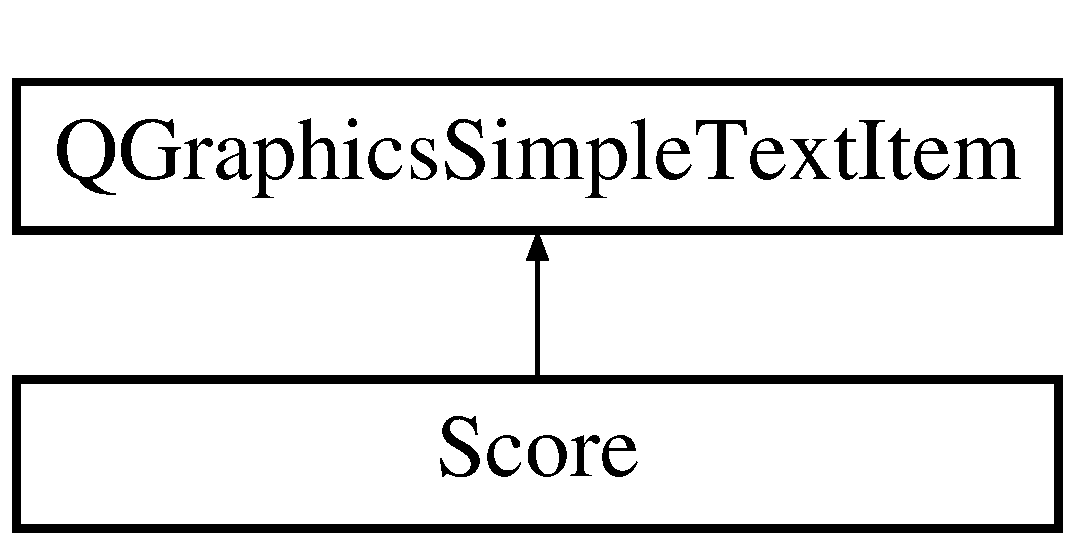
\includegraphics[height=2.000000cm]{classScore}
\end{center}
\end{figure}
\subsection*{Public Member Functions}
\begin{DoxyCompactItemize}
\item 
void \hyperlink{classScore_a32804ba9a847e58160e6e0cef46e1f25}{reset} ()
\item 
void \hyperlink{classScore_a3200804353edce251558f3a7ec40a195}{add} (int n)
\item 
int \hyperlink{classScore_a41b9a02dabc787db4d96021cf7b8b442}{get\-Score} () const 
\item 
void \hyperlink{classScore_ad4ffb432a3313d65f29b5448e61b6d50}{operator delete} (void $\ast$)
\end{DoxyCompactItemize}
\subsection*{Static Public Member Functions}
\begin{DoxyCompactItemize}
\item 
static \hyperlink{classScore}{Score} \& \hyperlink{classScore_a57963d0e399308580bd08c15f7ef52a2}{get} ()
\end{DoxyCompactItemize}


\subsection{Detailed Description}
Store the score in a game. 

Implements a counter of points. The class is implemented as a Singleton. Special care had to be taken to taken on object destruction, because the scene take ownership of its items and deletes them on destruction. 

\subsection{Member Function Documentation}
\hypertarget{classScore_a3200804353edce251558f3a7ec40a195}{\index{Score@{Score}!add@{add}}
\index{add@{add}!Score@{Score}}
\subsubsection[{add}]{\setlength{\rightskip}{0pt plus 5cm}void Score\-::add (
\begin{DoxyParamCaption}
\item[{int}]{n}
\end{DoxyParamCaption}
)}}\label{classScore_a3200804353edce251558f3a7ec40a195}
Add the given value to the score. \hypertarget{classScore_a57963d0e399308580bd08c15f7ef52a2}{\index{Score@{Score}!get@{get}}
\index{get@{get}!Score@{Score}}
\subsubsection[{get}]{\setlength{\rightskip}{0pt plus 5cm}{\bf Score} \& Score\-::get (
\begin{DoxyParamCaption}
{}
\end{DoxyParamCaption}
)\hspace{0.3cm}{\ttfamily [static]}}}\label{classScore_a57963d0e399308580bd08c15f7ef52a2}
Get the only instance of the score. \hypertarget{classScore_a41b9a02dabc787db4d96021cf7b8b442}{\index{Score@{Score}!get\-Score@{get\-Score}}
\index{get\-Score@{get\-Score}!Score@{Score}}
\subsubsection[{get\-Score}]{\setlength{\rightskip}{0pt plus 5cm}int Score\-::get\-Score (
\begin{DoxyParamCaption}
{}
\end{DoxyParamCaption}
) const\hspace{0.3cm}{\ttfamily [inline]}}}\label{classScore_a41b9a02dabc787db4d96021cf7b8b442}
Get the score. \hypertarget{classScore_ad4ffb432a3313d65f29b5448e61b6d50}{\index{Score@{Score}!operator delete@{operator delete}}
\index{operator delete@{operator delete}!Score@{Score}}
\subsubsection[{operator delete}]{\setlength{\rightskip}{0pt plus 5cm}void Score\-::operator delete (
\begin{DoxyParamCaption}
\item[{void $\ast$}]{}
\end{DoxyParamCaption}
)\hspace{0.3cm}{\ttfamily [inline]}}}\label{classScore_ad4ffb432a3313d65f29b5448e61b6d50}
Avoid deleting a score object. The singleton is stored in the scene, which takes ownership and deletes the item on destruction. Overwriting the delete-\/operator prevents this. \hypertarget{classScore_a32804ba9a847e58160e6e0cef46e1f25}{\index{Score@{Score}!reset@{reset}}
\index{reset@{reset}!Score@{Score}}
\subsubsection[{reset}]{\setlength{\rightskip}{0pt plus 5cm}void Score\-::reset (
\begin{DoxyParamCaption}
{}
\end{DoxyParamCaption}
)}}\label{classScore_a32804ba9a847e58160e6e0cef46e1f25}
Clear the score. 

The documentation for this class was generated from the following files\-:\begin{DoxyCompactItemize}
\item 
score.\-h\item 
score.\-cpp\end{DoxyCompactItemize}

\hypertarget{classScoreBoardManager}{\section{Score\-Board\-Manager Class Reference}
\label{classScoreBoardManager}\index{Score\-Board\-Manager@{Score\-Board\-Manager}}
}


Manage displaying the score board and name entry.  




{\ttfamily \#include $<$scoreboardmanager.\-h$>$}

Inheritance diagram for Score\-Board\-Manager\-:\begin{figure}[H]
\begin{center}
\leavevmode
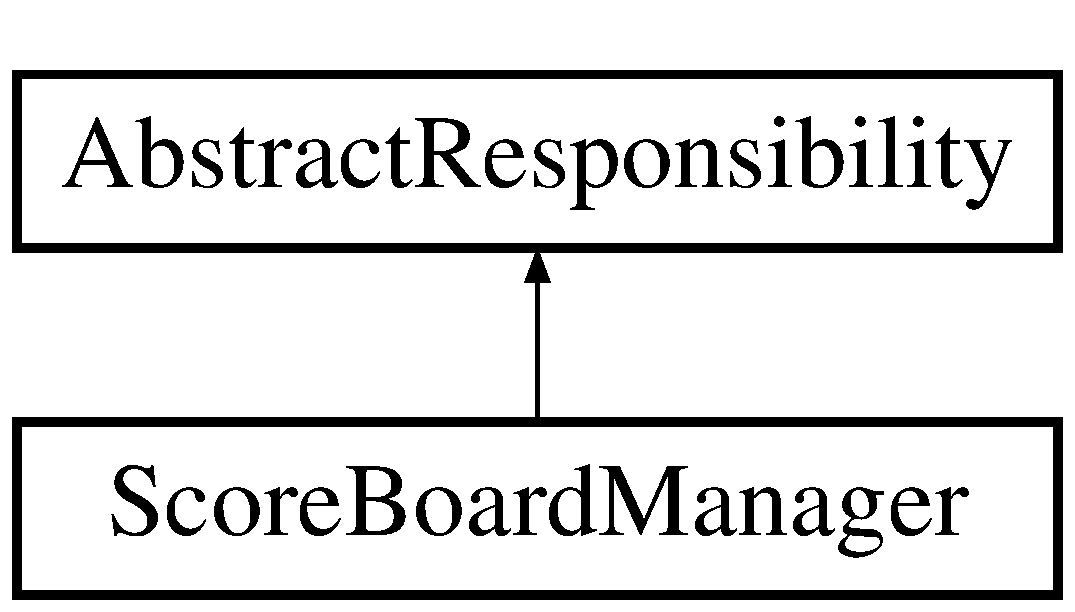
\includegraphics[height=2.000000cm]{classScoreBoardManager}
\end{center}
\end{figure}
\subsection*{Public Member Functions}
\begin{DoxyCompactItemize}
\item 
\hyperlink{classScoreBoardManager_a528501925af6d9d63186b29213af7456}{Score\-Board\-Manager} (\hyperlink{classDialog}{Dialog} $\ast$par)
\item 
void \hyperlink{classScoreBoardManager_a6dd53564ed29caaa34a043d62dbd113c}{handle\-Event} (\hyperlink{classEvent}{Event} $\ast$)
\end{DoxyCompactItemize}
\subsection*{Additional Inherited Members}


\subsection{Detailed Description}
Manage displaying the score board and name entry. 

Manage a score board, i.\-e., on pressing s the score board window is opened, on game over the score board with the ability to enter ones name is to be displayed. 

\subsection{Constructor \& Destructor Documentation}
\hypertarget{classScoreBoardManager_a528501925af6d9d63186b29213af7456}{\index{Score\-Board\-Manager@{Score\-Board\-Manager}!Score\-Board\-Manager@{Score\-Board\-Manager}}
\index{Score\-Board\-Manager@{Score\-Board\-Manager}!ScoreBoardManager@{Score\-Board\-Manager}}
\subsubsection[{Score\-Board\-Manager}]{\setlength{\rightskip}{0pt plus 5cm}Score\-Board\-Manager\-::\-Score\-Board\-Manager (
\begin{DoxyParamCaption}
\item[{{\bf Dialog} $\ast$}]{par}
\end{DoxyParamCaption}
)}}\label{classScoreBoardManager_a528501925af6d9d63186b29213af7456}
Hook ourself into the chain of responsibility, to watch out for s key presses or Out\-Of\-Lives\-Events. 

\subsection{Member Function Documentation}
\hypertarget{classScoreBoardManager_a6dd53564ed29caaa34a043d62dbd113c}{\index{Score\-Board\-Manager@{Score\-Board\-Manager}!handle\-Event@{handle\-Event}}
\index{handle\-Event@{handle\-Event}!ScoreBoardManager@{Score\-Board\-Manager}}
\subsubsection[{handle\-Event}]{\setlength{\rightskip}{0pt plus 5cm}void Score\-Board\-Manager\-::handle\-Event (
\begin{DoxyParamCaption}
\item[{{\bf Event} $\ast$}]{key}
\end{DoxyParamCaption}
)\hspace{0.3cm}{\ttfamily [virtual]}}}\label{classScoreBoardManager_a6dd53564ed29caaa34a043d62dbd113c}
Handle presses of s key and Out\-Of\-Live\-Events. 

Reimplemented from \hyperlink{classAbstractResponsibility_a14d885884ae4841dbe7c5824b986f2c9}{Abstract\-Responsibility}.



The documentation for this class was generated from the following files\-:\begin{DoxyCompactItemize}
\item 
scoreboardmanager.\-h\item 
scoreboardmanager.\-cpp\end{DoxyCompactItemize}

\hypertarget{classUi__Dialog}{\section{Ui\-\_\-\-Dialog Class Reference}
\label{classUi__Dialog}\index{Ui\-\_\-\-Dialog@{Ui\-\_\-\-Dialog}}
}
Inheritance diagram for Ui\-\_\-\-Dialog\-:\begin{figure}[H]
\begin{center}
\leavevmode
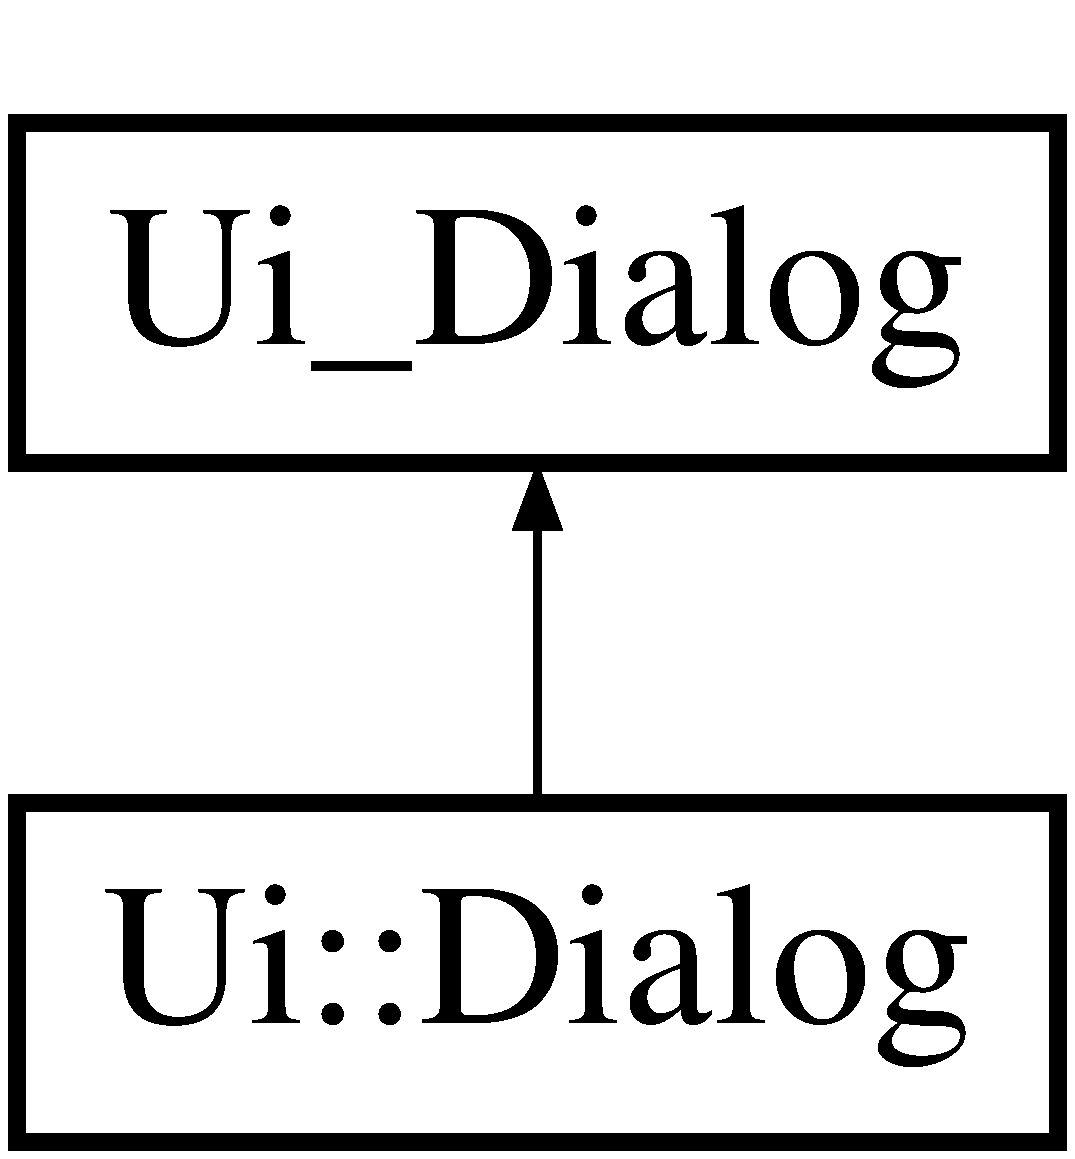
\includegraphics[height=2.000000cm]{classUi__Dialog}
\end{center}
\end{figure}
\subsection*{Public Member Functions}
\begin{DoxyCompactItemize}
\item 
\hypertarget{classUi__Dialog_a4f6a478c3ecdafabffb17b39cb26444a}{void {\bfseries setup\-Ui} (Q\-Dialog $\ast$\hyperlink{classDialog}{Dialog})}\label{classUi__Dialog_a4f6a478c3ecdafabffb17b39cb26444a}

\item 
\hypertarget{classUi__Dialog_afa0ccb6f716ca6178260522a193c250e}{void {\bfseries retranslate\-Ui} (Q\-Dialog $\ast$\hyperlink{classDialog}{Dialog})}\label{classUi__Dialog_afa0ccb6f716ca6178260522a193c250e}

\end{DoxyCompactItemize}


The documentation for this class was generated from the following file\-:\begin{DoxyCompactItemize}
\item 
ui\-\_\-dialog.\-h\end{DoxyCompactItemize}

\hypertarget{classUi__helpDialog}{\section{Ui\-\_\-help\-Dialog Class Reference}
\label{classUi__helpDialog}\index{Ui\-\_\-help\-Dialog@{Ui\-\_\-help\-Dialog}}
}
Inheritance diagram for Ui\-\_\-help\-Dialog\-:\begin{figure}[H]
\begin{center}
\leavevmode
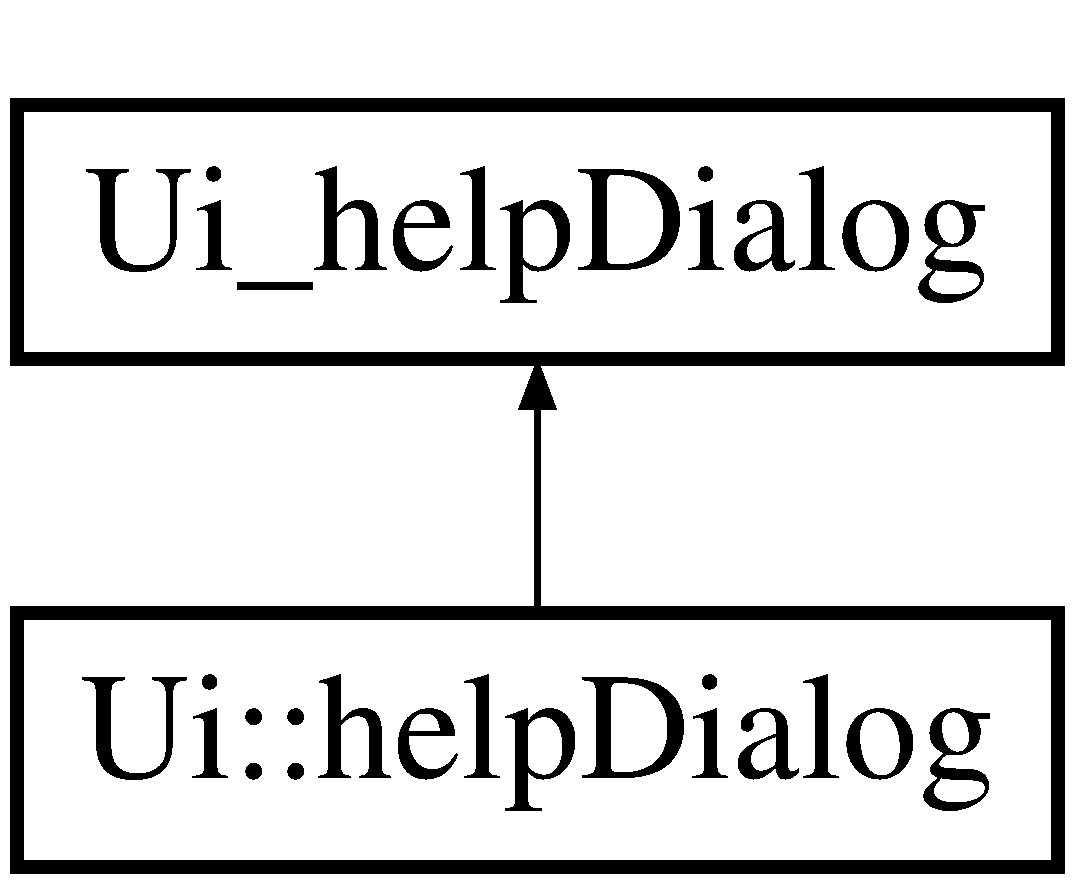
\includegraphics[height=2.000000cm]{classUi__helpDialog}
\end{center}
\end{figure}
\subsection*{Public Member Functions}
\begin{DoxyCompactItemize}
\item 
\hypertarget{classUi__helpDialog_a4074ac03760c68b2a4d9ba5e9aa47f4b}{void {\bfseries setup\-Ui} (Q\-Dialog $\ast$help\-Dialog)}\label{classUi__helpDialog_a4074ac03760c68b2a4d9ba5e9aa47f4b}

\item 
\hypertarget{classUi__helpDialog_a2f67a7a9b16bb22a264d312234c7e60d}{void {\bfseries retranslate\-Ui} (Q\-Dialog $\ast$help\-Dialog)}\label{classUi__helpDialog_a2f67a7a9b16bb22a264d312234c7e60d}

\end{DoxyCompactItemize}
\subsection*{Public Attributes}
\begin{DoxyCompactItemize}
\item 
\hypertarget{classUi__helpDialog_a1ee746becdf3250a159a36bc7e0d2724}{Q\-V\-Box\-Layout $\ast$ {\bfseries vertical\-Layout}}\label{classUi__helpDialog_a1ee746becdf3250a159a36bc7e0d2724}

\item 
\hypertarget{classUi__helpDialog_a67c0a23bf50b0edc6a2328499a0c412d}{Q\-Label $\ast$ {\bfseries label}}\label{classUi__helpDialog_a67c0a23bf50b0edc6a2328499a0c412d}

\item 
\hypertarget{classUi__helpDialog_aed3e82f455f7e3b3da6df686f1d6d200}{Q\-Text\-Browser $\ast$ {\bfseries text\-Browser}}\label{classUi__helpDialog_aed3e82f455f7e3b3da6df686f1d6d200}

\end{DoxyCompactItemize}


The documentation for this class was generated from the following file\-:\begin{DoxyCompactItemize}
\item 
ui\-\_\-helpdialog.\-h\end{DoxyCompactItemize}

\hypertarget{classUi__highScores}{\section{Ui\-\_\-high\-Scores Class Reference}
\label{classUi__highScores}\index{Ui\-\_\-high\-Scores@{Ui\-\_\-high\-Scores}}
}
Inheritance diagram for Ui\-\_\-high\-Scores\-:\begin{figure}[H]
\begin{center}
\leavevmode
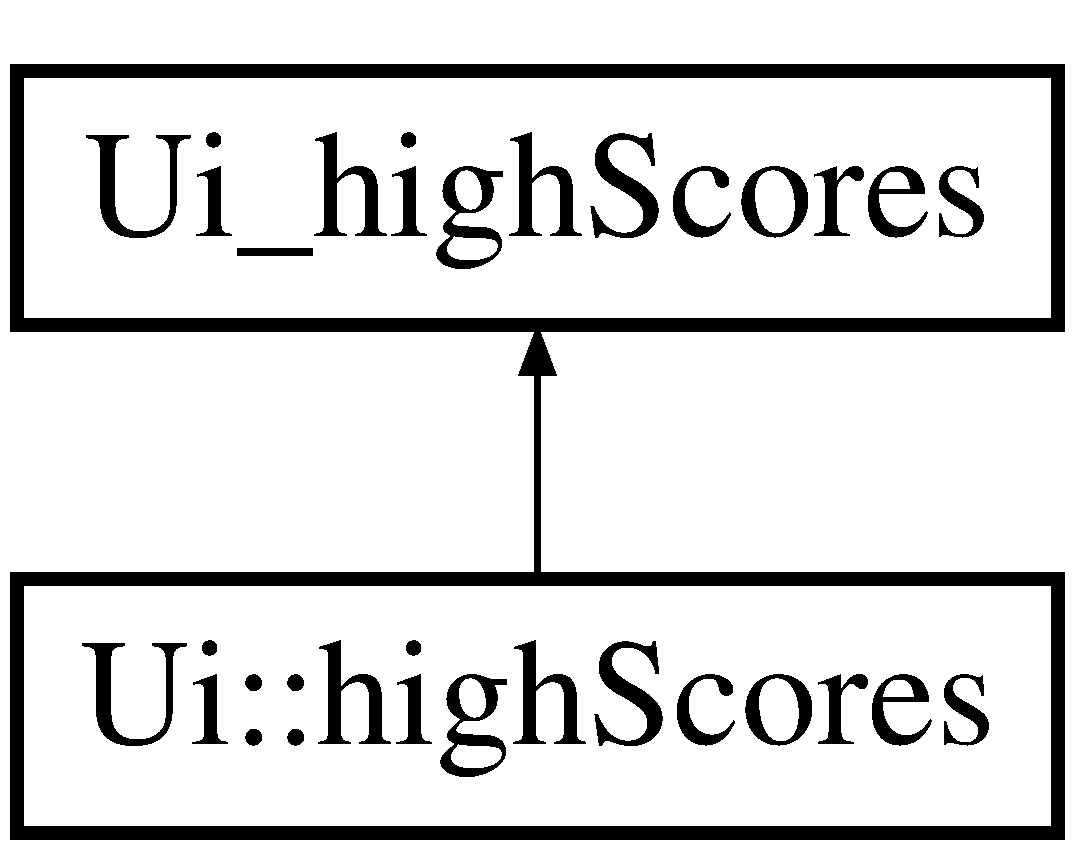
\includegraphics[height=2.000000cm]{classUi__highScores}
\end{center}
\end{figure}
\subsection*{Public Member Functions}
\begin{DoxyCompactItemize}
\item 
\hypertarget{classUi__highScores_a7789223a709e203477cb67b8d31b3d09}{void {\bfseries setup\-Ui} (Q\-Dialog $\ast$high\-Scores)}\label{classUi__highScores_a7789223a709e203477cb67b8d31b3d09}

\item 
\hypertarget{classUi__highScores_a318dbf59c03174ab36720fd547068864}{void {\bfseries retranslate\-Ui} (Q\-Dialog $\ast$high\-Scores)}\label{classUi__highScores_a318dbf59c03174ab36720fd547068864}

\end{DoxyCompactItemize}
\subsection*{Public Attributes}
\begin{DoxyCompactItemize}
\item 
\hypertarget{classUi__highScores_a54161485451a5ad1ced172052cb5d3a7}{Q\-V\-Box\-Layout $\ast$ {\bfseries vertical\-Layout}}\label{classUi__highScores_a54161485451a5ad1ced172052cb5d3a7}

\item 
\hypertarget{classUi__highScores_a2b10fee61ea84d2f71d41616e503ca9f}{Q\-Label $\ast$ {\bfseries label}}\label{classUi__highScores_a2b10fee61ea84d2f71d41616e503ca9f}

\item 
\hypertarget{classUi__highScores_adfeb2ab1e65bb13cbcda691bcef8272a}{Q\-Table\-Widget $\ast$ {\bfseries high\-Score\-Table}}\label{classUi__highScores_adfeb2ab1e65bb13cbcda691bcef8272a}

\end{DoxyCompactItemize}


The documentation for this class was generated from the following file\-:\begin{DoxyCompactItemize}
\item 
ui\-\_\-scoreboard.\-h\end{DoxyCompactItemize}

\addcontentsline{toc}{part}{Index}
\printindex
\end{document}
